

\section{动态放大器与相关电平移位技术}
\subsection{动态放大器的设计思想}
传统的低电压模拟电路设计中，增益和线性性能的提升通常依赖于增加晶体管的偏置电流和堆叠更多的晶体管。
由于供电电压较低，为了保持跨导不下降，电路中的晶体管往往处于亚阈值区工作状态，
此时晶体管的源极电流和栅极电压之间呈指数关系而非平方律。这样做虽然能够在低供电电压条件下提升电路的开环增益，
但是却是以牺牲电路的带宽为代价，
这样的模拟放大器频率响应较差，无法放大较高频率信号，器件无法以高压摆率工作\cite{tai2006bulkdrivenopamp,rajagopal2023subthresholdopamp}。
\par
对于静态低电压放大器来说，其供电电压一直加在晶体管的偏置回路上，也就是
无论有无信号输入，晶体管都需要持续地消耗电流以维持偏置点，这就导致了较高的静态功耗；这一特征在神经记录与生物前端低功耗放大器设计中尤为典型\cite{harrison2003neuralamp,chaya2020ultralowota,mukherjee2022ultralowia}。
但是对于ADC等器件来说，其工作状态呈现离散性和周期性，也就是很多时候处于空闲状态或者输入信号较小的状态，
此时如果持续地产生静态功耗就会造成能量的浪费。因此一个比较自然的想法就是设计一种
在特定时间阶段、有信号输入时才工作产生功耗，而在其他时间阶段则不工作或者功耗极低的放大器，
这就是动态放大器的设计思想。
\par
想要消除静态功耗，最直接的方式就是在没有信号输入时完全切断电流路径，这就需要在放大器中引入开关，
使得电路在没有信号输入时处于完全断电的状态；当有信号输入时，开关闭合，电路进入放大状态。
除此以外，电容作为储能元件也被引入到动态放大器中，
可以在无信号输入时由电源进行充电，在放大阶段为晶体管提供瞬态电流，
电容的充放电过程均产生动态功耗，形成瞬态增益。
开关电容电路的特征和动态放大器的设计思想高度契合，因此开关电容电路在动态放大器中被广泛采用。
\subsection{动态放大器基本机理}
动态放大器通常工作在离散时间多相时钟下。
在复位相位，输入信号被存储到采样电容，电源给储能电容充电；在放大相位，
输入信号接入动态放大器，同时电源断开，而由储能电容给工作晶体管供电，形成瞬态增益。
图\ref{fig:DA}展示了一个基本动态放大器的原理图和时序示例。
与静态 OTA 相比，其本质差异在于“瞬态增益”替代“持续偏置增益”。
这使其在低占空比系统中具有天然能效优势，但也使性能更依赖时序与寄生条件。

\begin{figure}[htbp]
    \centering
    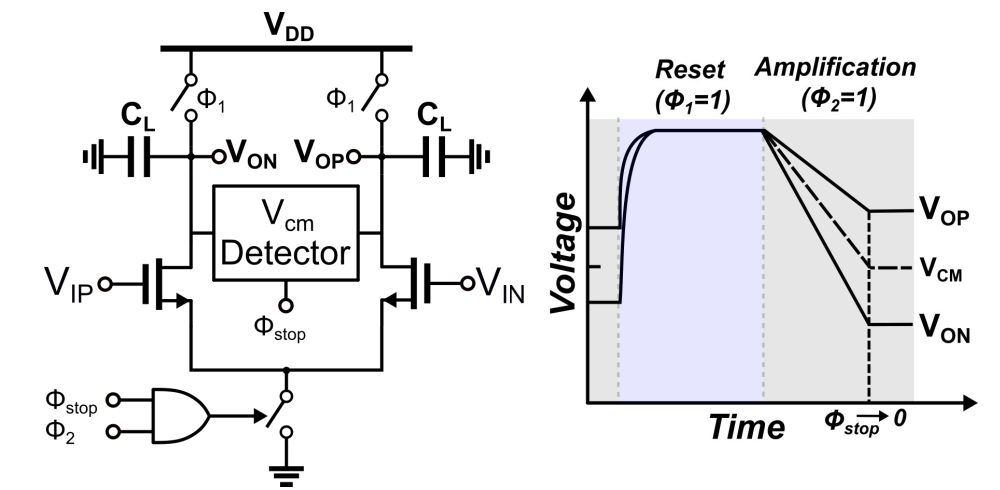
\includegraphics[width=0.8\textwidth]{doc_thesis/figs/04/基本动态放大器.png}
    \caption{\ptheadingfont{基本动态放大器的原理图和时序图}}
    \label{fig:DA}
\end{figure}


从系统角度看，动态放大器适合用于开关电容积分器、
离散时间噪声整形环路和低带宽高分辨数据转换器。
典型优势可概括为：(1) 静态功耗极低；(2) 电路结构与数字时钟协同紧密；
(3) 在中低带宽下具有较高功耗性能比。
对应不足包括：(1) 对时钟相位误差敏感；(2) 动态节点误差源复杂；
(3) 低电压下工作区间受限，易出现线性退化。

\subsection{FIA：浮动反相放大器}
传统的的动态放大器需要额外设计共模电压检测器，增加了电路结构复杂度，同时也有
增益不高，PVT稳定性不足的问题。
数字电路中的反相器（Inverter）在工作过程中，
两个MOS管无法同时导通，无法形成静态回路，因而也不产生静态功耗，只有在输入信号发生变化时才会产生动态功耗。
这种工作特点和动态放大器的设计思想高度契合，因此研究者们将反相器引入到动态放大器的设计中，形成了FIA（Floating Inverter Amplifier）结构。
\par
FIA（Floating Inverter Amplifier）利用互补金属氧化物半导体（Complementary Metal-Oxide-Semiconductor, CMOS）反相器作为高跨导核心，
通过“浮动”工作方式在放大相位获得较高等效增益，
其原理图和时序图如图\ref{fig:FIA}所示。
FIA同样存在复位（Reset）和放大（Amplification）两个阶段，
复位时由电源给负载电容充电，放大时负载电容放电形成动态电流进行放大。
基本动态放大器不同，FIA由于对称的结构设计和开关分布，
使得其不需要添加额外的共模电压检测部分以切断静态电流，
在放大阶放电完毕后静态电流自然消失，有着更出色的共模抑制能力。
该结构在近年低功耗 ADC 与 CDC 研究中被广泛采用
\cite{wang2021sefiamod,wu2025lvfia,tang2020zoomcdc}。
其价值在于能以较低能耗换取较高放大效率，
但工程上需重点控制共模变化、时钟耦合与开关注入带来的增益波动。

\begin{figure}[htbp]
    \centering
    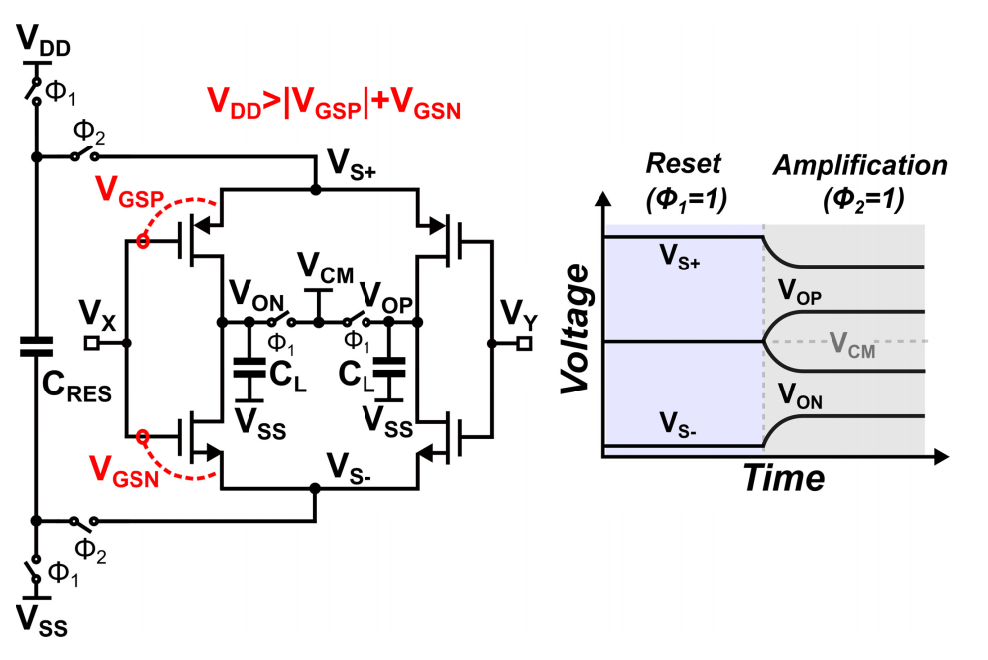
\includegraphics[width=0.8\textwidth]{doc_thesis/figs/04/FIA.png}
    \caption{\ptheadingfont{FIA的原理图和时序图}}
    \label{fig:FIA}
\end{figure}

\subsection{SEFIA：摆幅增强型 FIA}

SEFIA（Swing-Enhanced FIA）可视为对 FIA 的摆幅与线性增强，
其原理图和时序图如图\ref{fig:SEFIA}所示。
其主要思路是通过结构与时序协同，
扩大有效线性工作区并缓解大信号条件下的压缩失真。
在普通的浮动反相放大器FIA中，由于从VDD到VSS之间存在 p 沟道金属氧化物半导体晶体管（P-channel Metal-Oxide-Semiconductor, PMOS）和 n 沟道金属氧化物半导体晶体管（N-channel Metal-Oxide-Semiconductor, NMOS）堆叠，
这限制了模拟放大器的输出电压摆幅。而在SEFIA中，采用了自动归零技术，
使得PMOS和NMOS分别采用了独立的偏置电压，
这样的设计提高了放大器的线性输出摆幅，不过作为代价，
由于PMOS和NMOS中间跨接了一个电容器CI，电源电压相比于FIA要更大一些，
这使得SEFIA难以满足低供电电压条件下的应用。
相关研究表明，SEFIA 在微瓦级功耗条件下能够有效支持高分辨
离散时间调制器前端\cite{wang2021sefiamod}。
但这类结构通常引入更复杂的相位控制与版图约束，对实现一致性提出更高要求。

\begin{figure}[htbp]
    \centering
    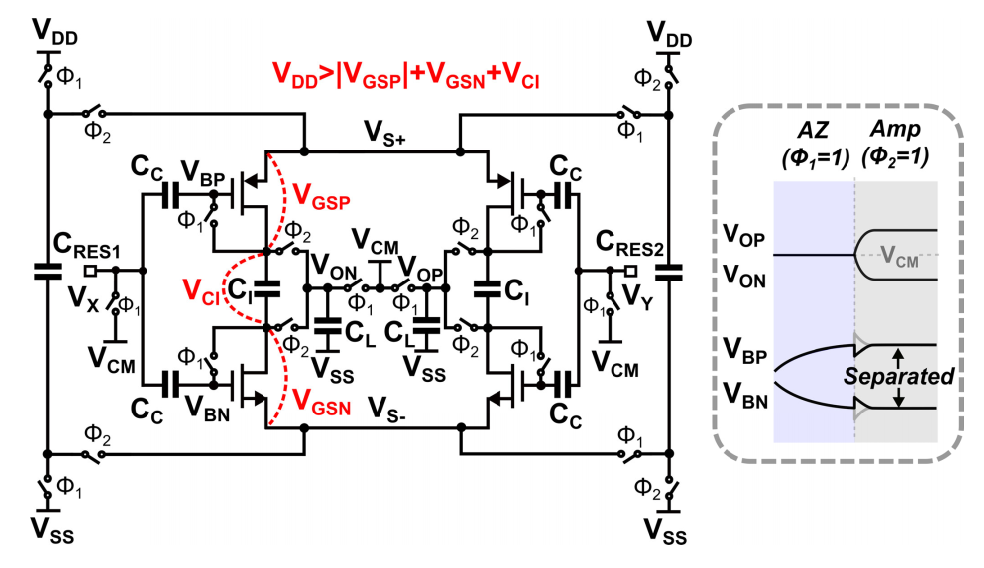
\includegraphics[width=0.8\textwidth]{doc_thesis/figs/04/SEFIA.png}
    \caption{\ptheadingfont{SEFIA的原理图和时序图}}
    \label{fig:SEFIA}
\end{figure}
根据上述分析，目前已有的动态放大器设计分别存在一些不足。
FIA 结构虽然能在低功耗条件下提供较高增益，但其输入共模范围和输出摆幅受限，导致线性性能下降；
SEFIA 通过增加偏置电压提升线性，但这使其难以适应亚 1.2V 的低压环境；
两者都对时钟抖动和非重叠时序敏感，缺乏有效的误差抑制机制。
如何设计一种低供电电压、高动态范围、高增益和精度的动态放大器以适用于物联网、传感器、生物医药领域的应用，
是本论文重点探讨的课题。
\subsection{LVFIA：低压浮动反相放大器}

LVFIA 面向亚 1.2V 乃至更低供电环境，
核心目标是在有限电压余量内维持可接受的增益与线性\cite{wu2025lvfia},
其原理图和时序图如图\ref{fig:LVFIA图示}所示。
分析电路可知，在一般FIA和SEFIA的基础上，图中所示的LVFIA电路同样使用了
CRES作为储能电容，在初始化阶段时由电源对其充电，
放大阶段时电容放电偏置晶体管；同时对称的电路结构以及负载电容CL的设置
确保了电路不需要额外共模反馈，在复位阶段能自动稳定到共模电压VCM。
具体改进的部分包含以下几点：其一，LVFIA在SEFIA的基础上，
去掉了浮空电容CI并舍弃了推挽的电路结构，将每个晶体管的偏置回路物理分离，
例如由图1中可见给每个PMOS都设置了独立的VSS，给每个NMOS都设置了独立的VDD，
这样做最直接且重要的影响就是解除了偏置时PMOS和NMOS之间电压关系的耦合性，
晶体管不再堆叠而给电源电压造成负担，降低了对电源电压大小的要求；
其二，在FIA和SEFIA的两相操作（复位阶段、放大阶段）的基础上，
LVFIA引入了三相操作，在复位阶段和放大阶段的中间加入放电和自归零阶段
（auto zero），在这一阶段通过电容CC1和CC2放电建立了PMOS和NMOS晶体管的
偏置电压VBP和VBN，并且由于此时PMOS和NMOS的栅极和漏极直接相连，
形成了一个二极管（Diode）结构，所以达到稳态后两者的栅源电压VGS很大程度上
和电源电压无关，这一点保证了即使电源电压有波动的情况下放大器偏置点仍然保持稳定，
消除了失调电压。总结来说，LVFIA的电路结构在FIA和SEFIA的基础上，
物理隔离了各个晶体管的偏置回路，去掉了浮空电容CI，
消除了晶体管堆叠对电源电压造成的抬升；同时引入自归零相，
在该阶段实现了对晶体管的稳定偏置，减少电源电压波动造成的偏置点的偏移。

\begin{figure}[htbp]
\centering
\subfigure[LVFIA的原理图]{
		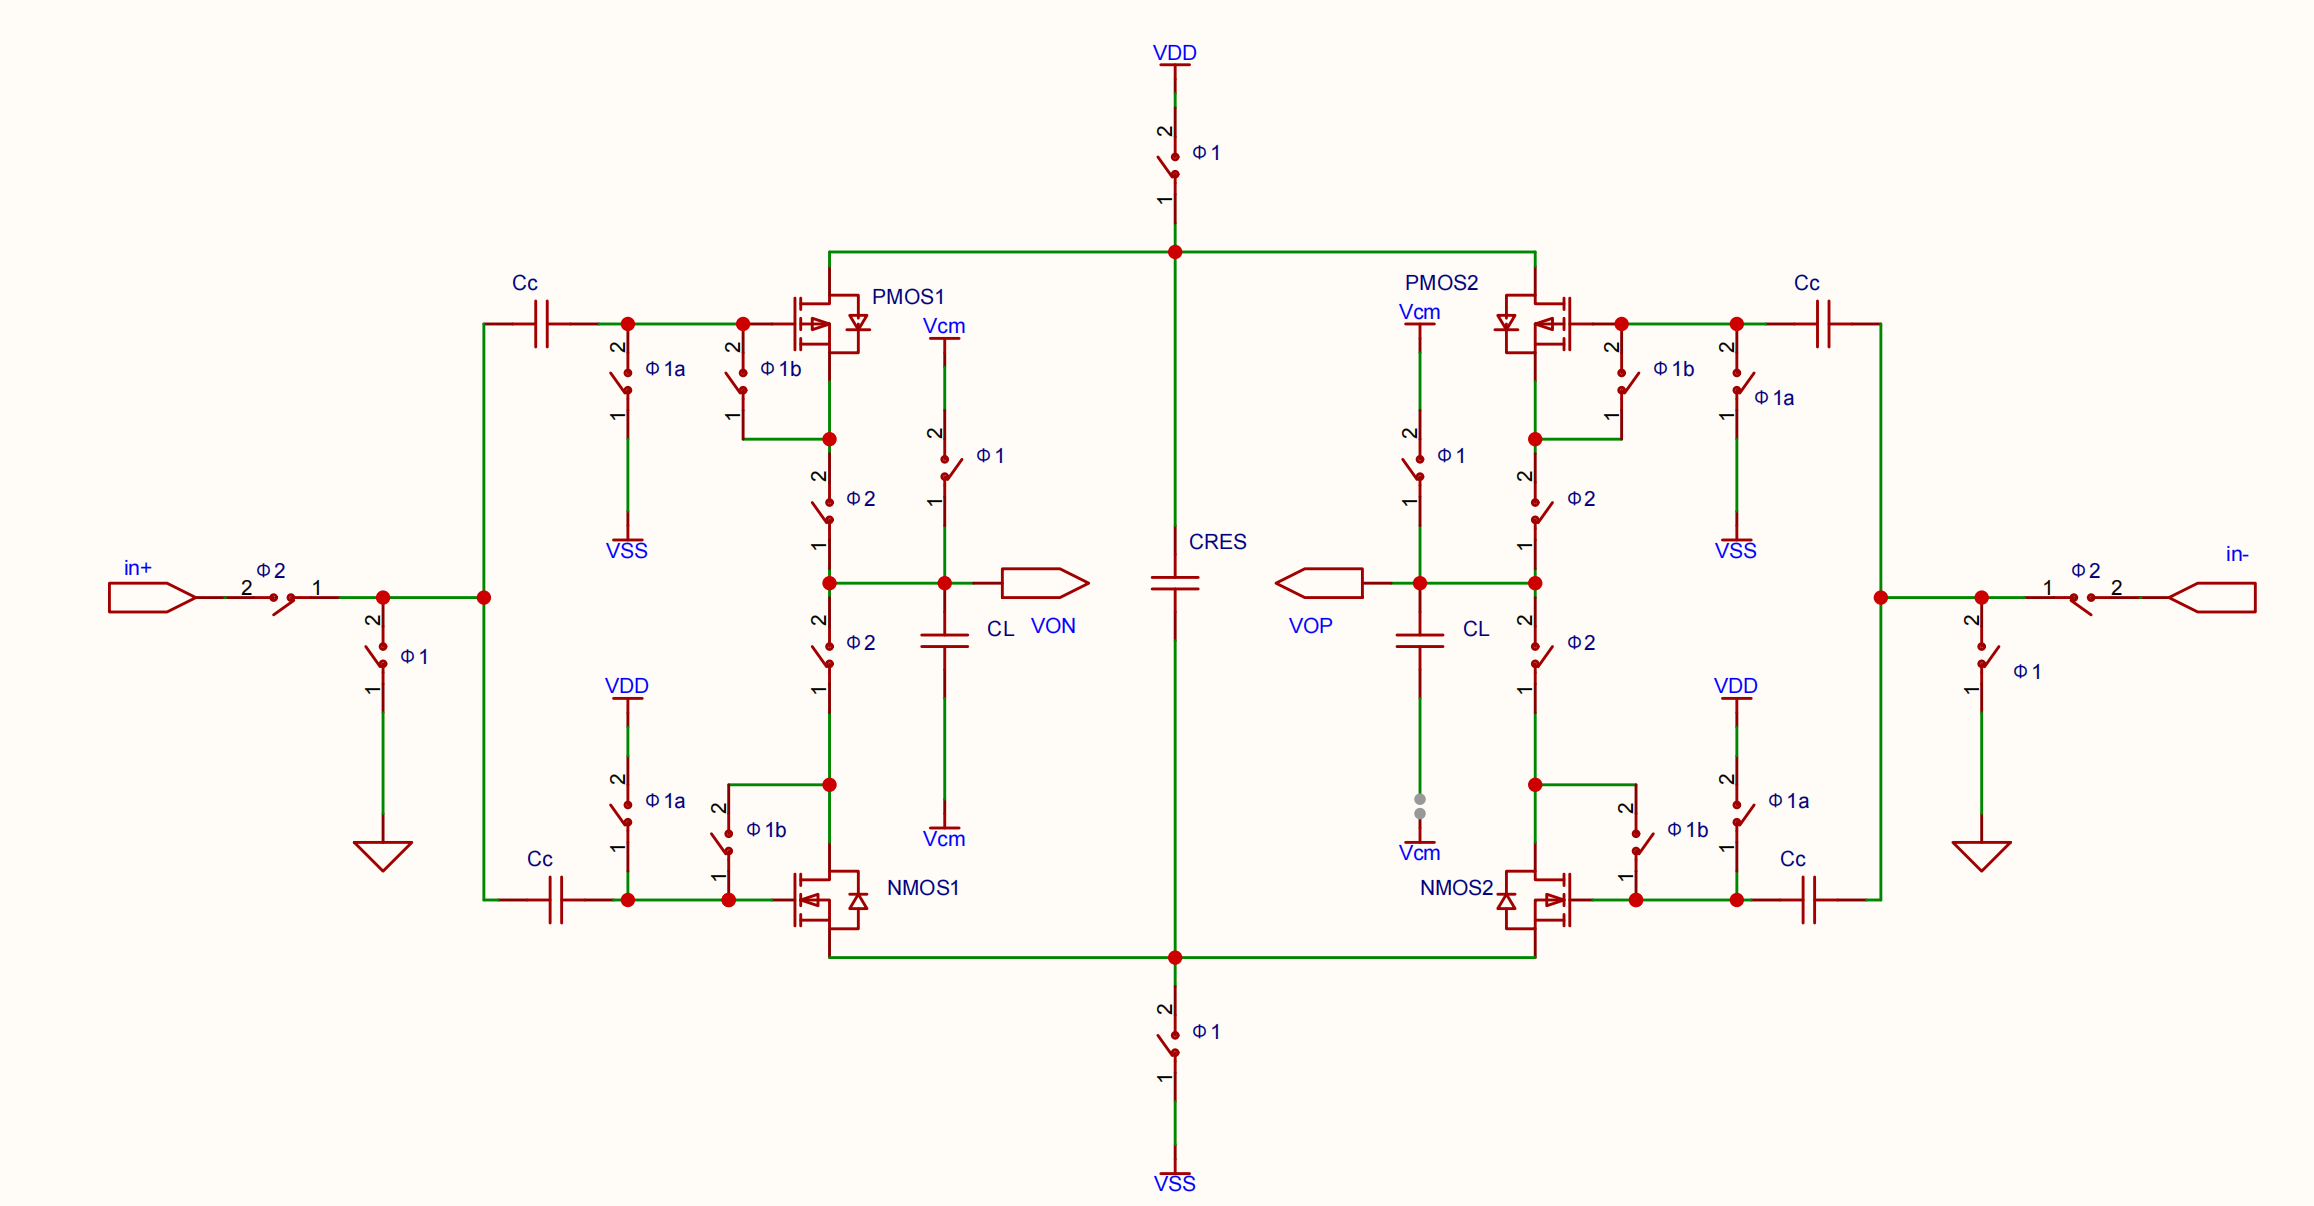
\includegraphics[width=0.48\textwidth]{doc_thesis/figs/04/LVFIA.png}}
\hfill
\subfigure[LVFIA的时序图]{
		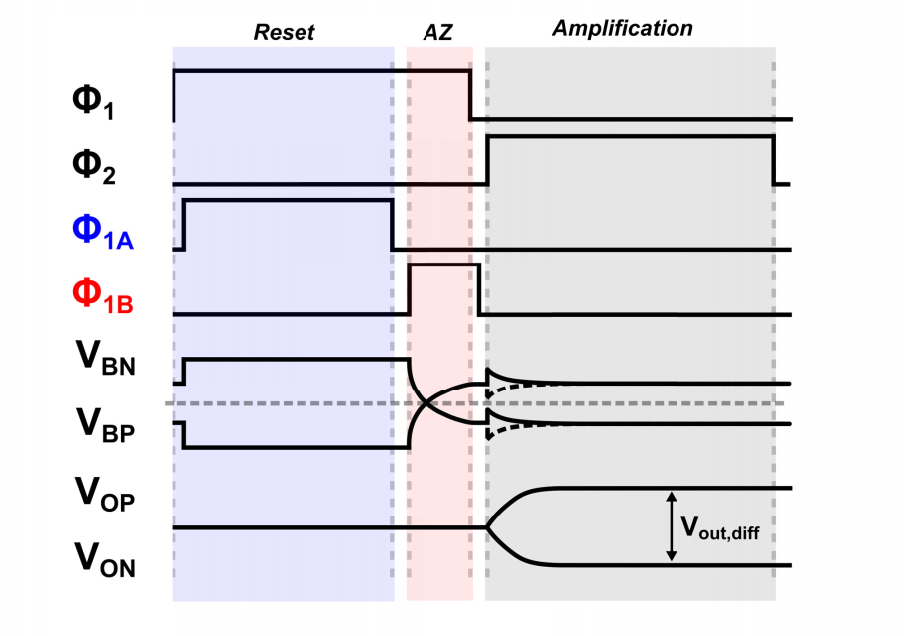
\includegraphics[width=0.48\textwidth]{doc_thesis/figs/04/LVFIA_timing.png}}
\caption{LVFIA的原理图和时序图}
    \label{fig:LVFIA图示}
\end{figure}



\subsection{基于动态放大器的闭环SC积分器电路}
\subsubsection{SC放大器的基本结构}
开关电容放大器使用开关信号和电容器件来实现放大功能，
基本的开关电容放大器结构如图\ref{fig:SC_amplifier}所示，
其中P1代表采样阶段，将输入信号电压采集到电容${C_1}$上；
P2代表放大阶段，此时开关闭合形成反馈回路，电容${C_2}$与放大器输入端形成电荷重分配，实现放大功能，
该阶段的等效电路如图\ref{fig:SC_amplifier_equivalent}所示。
在闭环放大器中，SC放大器采用负反馈结构，使用开关和电容器件
（类比普通放大器中的电阻器件）形成反馈回路，
能够实现增益、带宽和功耗的灵活调节。

\begin{figure}
    \centering
    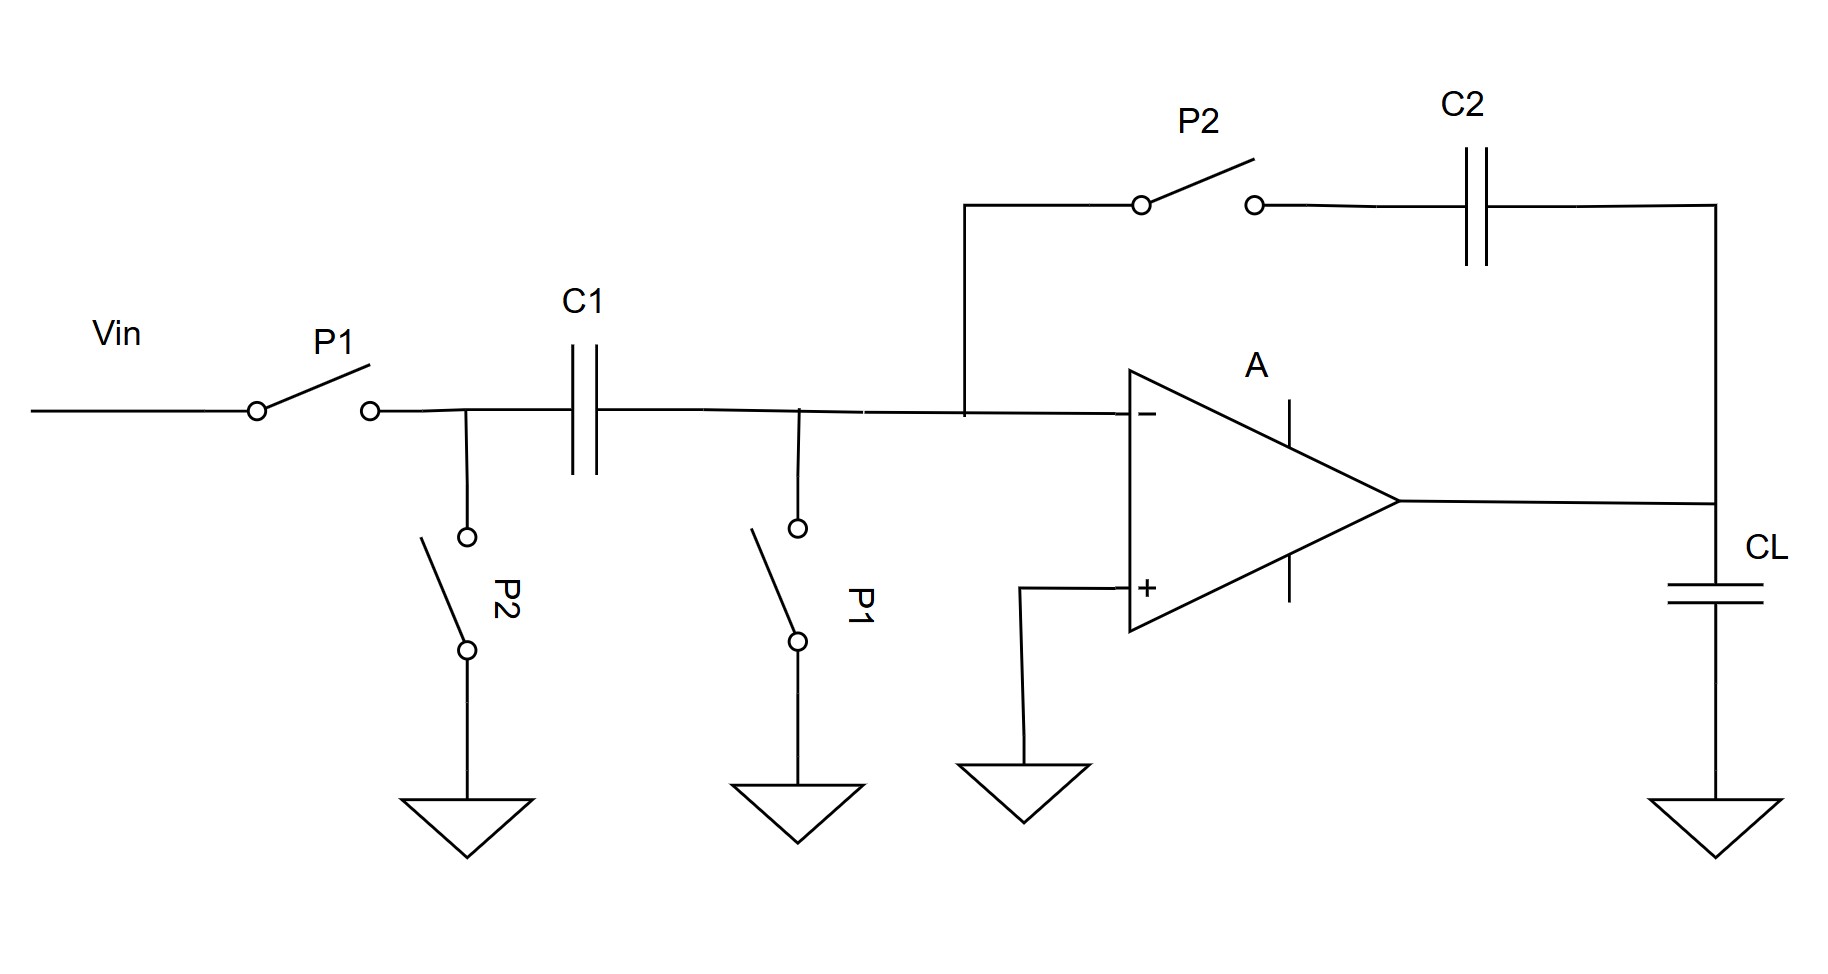
\includegraphics[width=0.8\textwidth]{doc_thesis/figs/04/SC放大器.png}
    \caption{\ptheadingfont{基本的开关电容放大器结构}}
    \label{fig:SC_amplifier}
\end{figure}

\begin{figure}
    \centering
    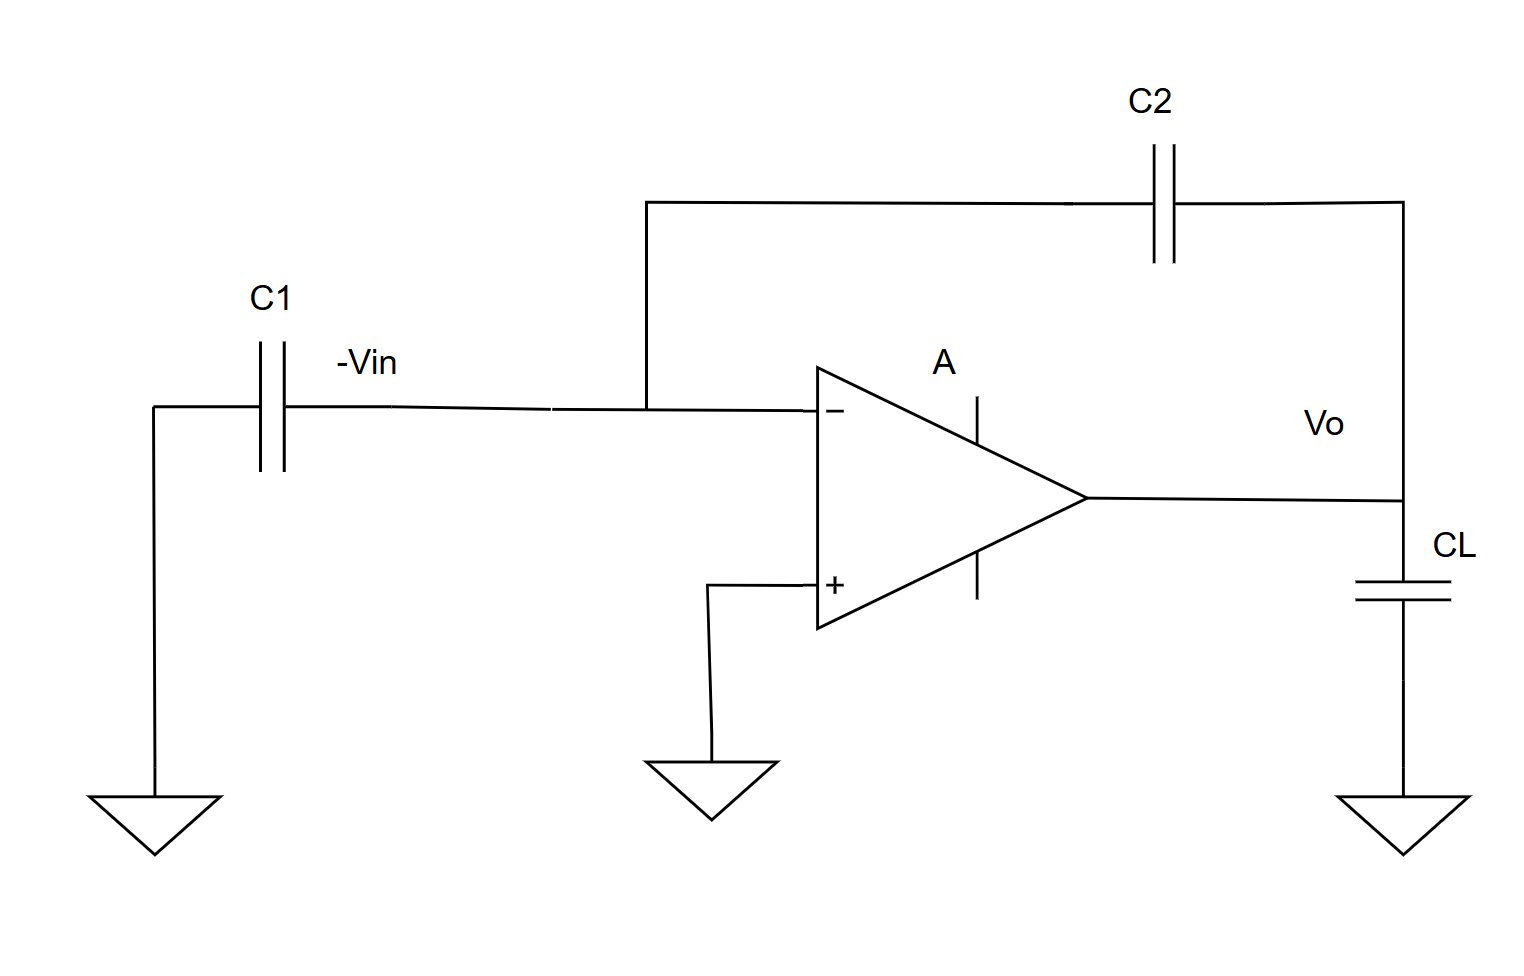
\includegraphics[width=0.8\textwidth]{doc_thesis/figs/04/SC放大器闭合开关.png}
    \caption{\ptheadingfont{P2阶段的开关电容放大器等效电路}}
    \label{fig:SC_amplifier_equivalent}
\end{figure}

经过理论分析，SC放大器的增益${\frac{V_o}{V_{in}} }$表达式为

\begin{equation}
    \frac{V_o}{V_{in}} = \frac{C_1}{C_2}\cdot\frac{1}{1+\frac{1}{T} }
    \label{equa:SC_amplifier_1}
\end{equation}

其中T为环路增益，也即
\begin{equation}
    T = \frac{C_2}{C_1}\cdot A_0
    \label{equa:SC_amplifier_2}
\end{equation}

当使用的是理想运放时，其开环增益$A_0$趋近于无穷大，
$C_1$采样到的电荷全部转移到电容$C_2$上，运放的反相输入端电平为0，形成了虚地点。此时上式退化为
\begin{equation}
    \frac{V_o}{V_{in}} \rightarrow \frac{C_1}{C_2}
\end{equation}

\subsubsection{基于LVFIA的SC闭环放大器}
SC放大器的外围电路为开关电容电路，其动态特性和LVFIA的设计思想高度契合，
主要体现在两个相位阶段和LVFIA的一致性上，因此基于LVFIA的SC放大器具有天然的优势。
基于LVFIA，可以设计如图\ref{fig:LVFIA_integrator}所示的积分器电路,
其本质是将前面所述的基本SC放大器中的运算放大器部分替换为LVFIA结构，
这也是LVFIA等动态放大器最基本的应用电路之一。在这个闭环负反馈电路中，
开关电容器件取代了电阻形成了反馈回路。通过控制电容比值${\frac{C_1}{C_2} }$
能够控制电路的整体增益，同时由于电容的充放电过程会产生动态功耗，
因此该电路也具有动态放大器的特征。
\par
参考文献\cite{wu2025lvfia}中对LVFIA的小信号分析，其开环增益可写为跨导与输出电阻的乘积：
\begin{equation}
    A_{0,\mathrm{LVFIA}} = g_{m,\mathrm{eq}} \cdot R_{out,\mathrm{eq}}
\end{equation}
其中等效跨导由反相器的NMOS与PMOS并联贡献给出：
\begin{equation}
    g_{m,\mathrm{eq}} \approx g_{mn}+g_{mp}
\end{equation}
对级联结构，单支路输出电阻可近似写为：
\begin{equation}
    R_{on,\mathrm{cas}} \approx g_{mn,c}\,r_{on}\,r_{on,c},\qquad
    R_{op,\mathrm{cas}} \approx g_{mp,c}\,r_{op}\,r_{op,c}
\end{equation}
因此差分等效输出电阻可表示为：
\begin{equation}
    R_{out,\mathrm{eq}} \approx R_{on,\mathrm{cas}} \parallel R_{op,\mathrm{cas}}
\end{equation}
将上式代入可得LVFIA开环增益近似：
\begin{equation}
    A_{0,\mathrm{LVFIA}} \approx (g_{mn}+g_{mp})\cdot
    \left[\left(g_{mn,c}\,r_{on}\,r_{on,c}\right)\parallel
    \left(g_{mp,c}\,r_{op}\,r_{op,c}\right)\right]
\end{equation}

当LVFIA用于开关电容积分器时，反馈因子可写为
\begin{equation}
    \beta=\frac{C_2}{C_1+C_2}
\end{equation}
闭环增益满足
\begin{equation}
    A_{cl}=\frac{A_{0,\mathrm{LVFIA}}}{1+\beta A_{0,\mathrm{LVFIA}}}
\end{equation}
进一步可得单级积分器从输入到输出的传输关系：
\begin{equation}
    \frac{V_{out}}{V_{in}}
    =-\frac{C_1}{C_2}\cdot
    \frac{A_{0,\mathrm{LVFIA}}}{A_{0,\mathrm{LVFIA}}+1+\frac{C_1}{C_2}}
\end{equation}
在理想高增益极限下（$A_{0,\mathrm{LVFIA}}\rightarrow\infty$），上式退化为
\begin{equation}
    \frac{V_{out}}{V_{in}} \rightarrow -\frac{C_1}{C_2}
\end{equation}
对应有限增益导致的闭环误差近似为
\begin{equation}
    \varepsilon_A
    \approx \frac{1+\frac{C_1}{C_2}}{A_{0,\mathrm{LVFIA}}}
\end{equation}


由上述分析可知，为了减小增益误差，需要一个足够高的开环增益$A_{0,\mathrm{LVFIA}}$。
然而对于LVFIA来说，其在低压条件下的增益和线性仍然受限，尤其在输入共模电压接近电源轨时，增益会显著下降。
通常的解决方法是引入Cascode结构，通过直接提高跨导以提升开环增益，但这会增加电路复杂度和功耗，同时
Cascode结构的引入也会增加对电源电压的要求，降低电路的适用范围。
因此，如何在保持LVFIA低压适应性的同时提升其增益和线性，是本论文后续研究的重点之一。

\begin{figure}[htbp]
    \centering
    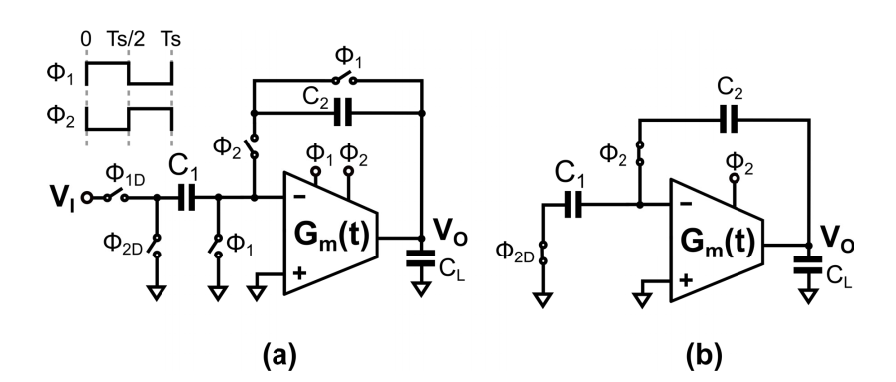
\includegraphics[width=0.8\textwidth]{doc_thesis/figs/04/基于LVFIA的积分器.png}
    \caption{\ptheadingfont{基于LVFIA的开关电容积分器电路设计}}
    \label{fig:LVFIA_integrator}
\end{figure}

\subsection{CLS技术及其在动态放大器中的作用}

\subsubsection{CLS基本思想}
前面所述的SC放大器，其闭环增益和反馈比${\frac{C_1}{C_2}}$存在误差的主要原因是：
在运放增益A有限的情况下，电路最终达到平衡后，放大器输入端的电压不再是虚地，而是存在一个小的电压偏移。
直接提升放大器的开环增益A是提升闭环增益的一个直接方法，但这通常会增加电路复杂度和功耗。
自然而然地，一个更好的想法是：不改变运放本身，而是通过外围电路设计和
开关电容操作来设法降低放大器输入端的电压偏移，
从而提升闭环增益使之更加接近理想值${\frac{C_1}{C_2}}$。
相关电平移位（Correlated Level Shifting, CLS）旨在通过在特定时钟相位内执行
受控电平重定位，通过间接的方式提高SC放大器中LVFIA的等效增益，其全程只通过
开关电容网络进行电荷重分配，而无需增加持续偏置电流或晶体管堆叠，为上述思路提供了
一种具体的解决方案。
CLS技术的核心并非静态抬升某个节点电平，
而是在与采样/放大过程相关的时钟相位内执行受控电平重定位，使移位引入的误差项与主信号链路保持相关，
从而在后续积分、噪声整形或反馈中被部分抑制\cite{essam2010twophasecls,hu2022mashcls,meng2023jssc_mash}。


\subsubsection{CLS基本原理}
CLS给SC放大器带来的主要变化可以概括为在基本动态放大器的输出端和整体的闭环放大器输出端之间
引入电平移位电容$C_{CLS}$，以及一个受控的电平移位阶段，
在该阶段通过开关电容网络对关键节点进行电荷重分配，电平移位电容串联在两者之间进行隔离
而非一般SC放大器的直接相连。其中对于电平移位电容来说，基本动态放大器的输出端电平
低于闭环放大器输出端电平，因此电平移位电容的正极接在基本动态放大器的输出端，负极接在闭环放大器输出端。
这样的设计会带来几个直接的影响：其一，CLS通过电荷重分配改变了动态放大器进入放大相时的工作点，
在一瞬间降低了基本动态放大器的输出电压，使输入对管和负载器件落在更有利的瞬时跨导区间，
从而提升了放大器的增益和线性性能；其二，一个电平移位电容${C_{CLS}}$隔离了
基本放大器的输出端和电路整体的输出端，电路整体输出电压不再直接是基本动态放大器的输出端
电压，更准确地，是基本动态放大器输出端电压与电平移位电容上电荷重分配引起的电压变化的叠加，
这一变化除了带来增益提升之外，还把有限开环增益和电源轨限制导致的增益误差映射为可被后级处理的相关误差，
降低了由于输出电压接近电源轨时导致的非线性失真，提高了放大器输出的线性范围。
\par
从电路机理看，CLS通过开关电容网络在特定相位完成电荷再分配或节点预充，
改变动态放大器进入放大相时的初始工作点，使输入对管和负载器件落在更有利的瞬时跨导区间；
同时把有限开环增益导致的残差映射为可被后级处理的相关误差，降低非线性外显\cite{hung2016averagingcls,kumar2022cascodedfia}。
因此，CLS属于“利用离散时间自由度换取等效增益与线性”的方法，
在不显著增加静态功耗与晶体管堆叠的前提下提升低压可用性\cite{hu2022mashcls,meng2023jssc_mash}。

\subsubsection{CLS执行过程}

典型CLS执行可归纳为三步：其一，采样/复位相建立输入电荷与参考共模,
输入电压被采样到采样电容上，同时反馈电容${C_2}$、电平移位电容${C_{CLS}}$和输出端
负载电容${C_L}$全部复位；
其二，放大相时采样电容接入放大器输入端，动态放大器进入放大相，
采样电容与反馈电容连接形成电荷重分配网络，电平移位电容${C_{CLS}}$和负载电容${C_L}$
并联，此时整体放大器形成一个基本的闭环SC放大器结构，和之前论文中提到的开关电容积分器结构
没有本质的区别；
其三，电平移位相时，通过开关控制，电平移位电容串联接入放大器输出端和负载电容之间，
降低了放大器的输入输出电压，提高采样电容电荷转移。对于整体应用电路例如ADC，
电路在电平移位相的最后采集放大的电压信号，完成信号传递，
并将移位相关误差压入后级噪声整形或数字补偿链路\cite{essam2010twophasecls,li2024crcls}。
在工程实现上，非重叠时钟精度、开关注入以及寄生失配会直接决定CLS增益提升是否可兑现，
因此CLS设计本质是电路、时序与版图协同优化\cite{hung2016averagingcls,liu2020pingpongcls}。

\begin{figure}[htbp]
\centering
\subfigure[CLS初步放大阶段时的电路连接图]{
		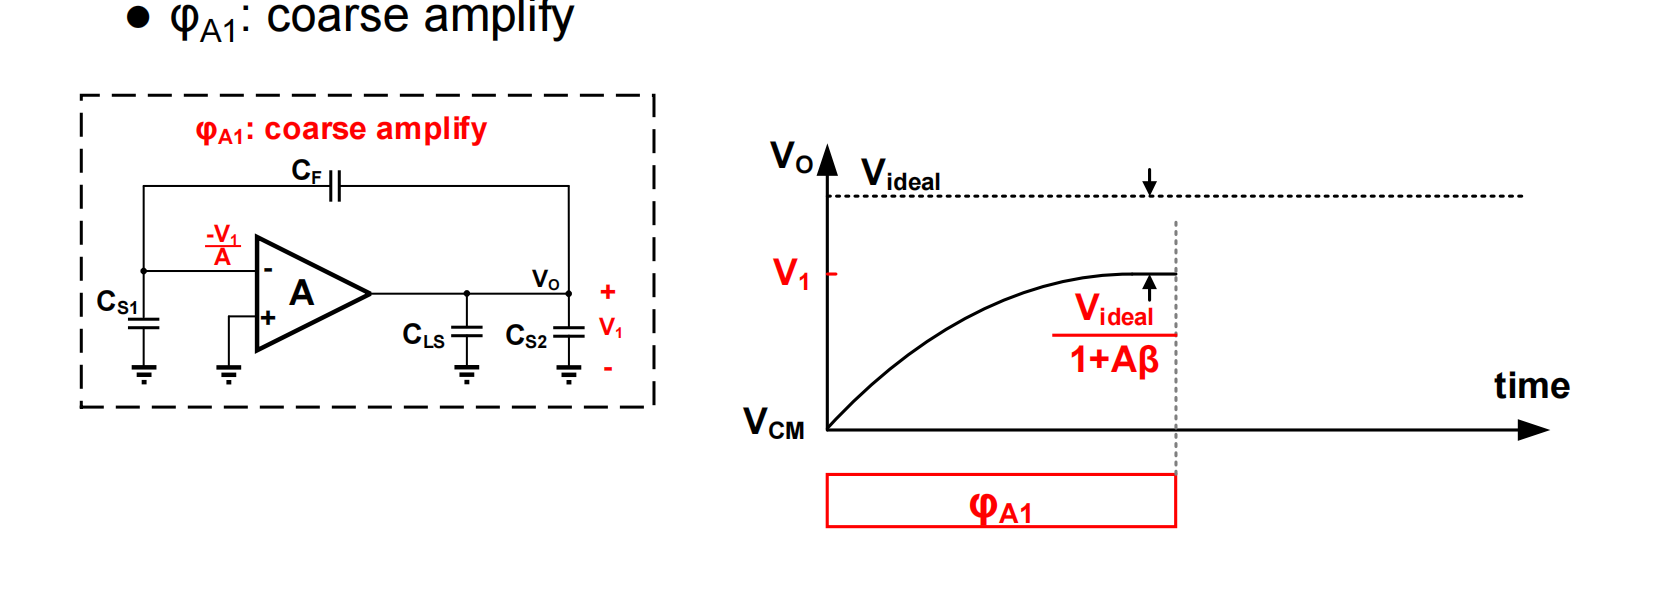
\includegraphics[width=0.48\textwidth]{doc_thesis/figs/04/CLS阶段1.png}}
\hfill
\subfigure[CLS电平移位阶段时的电路连接图]{
		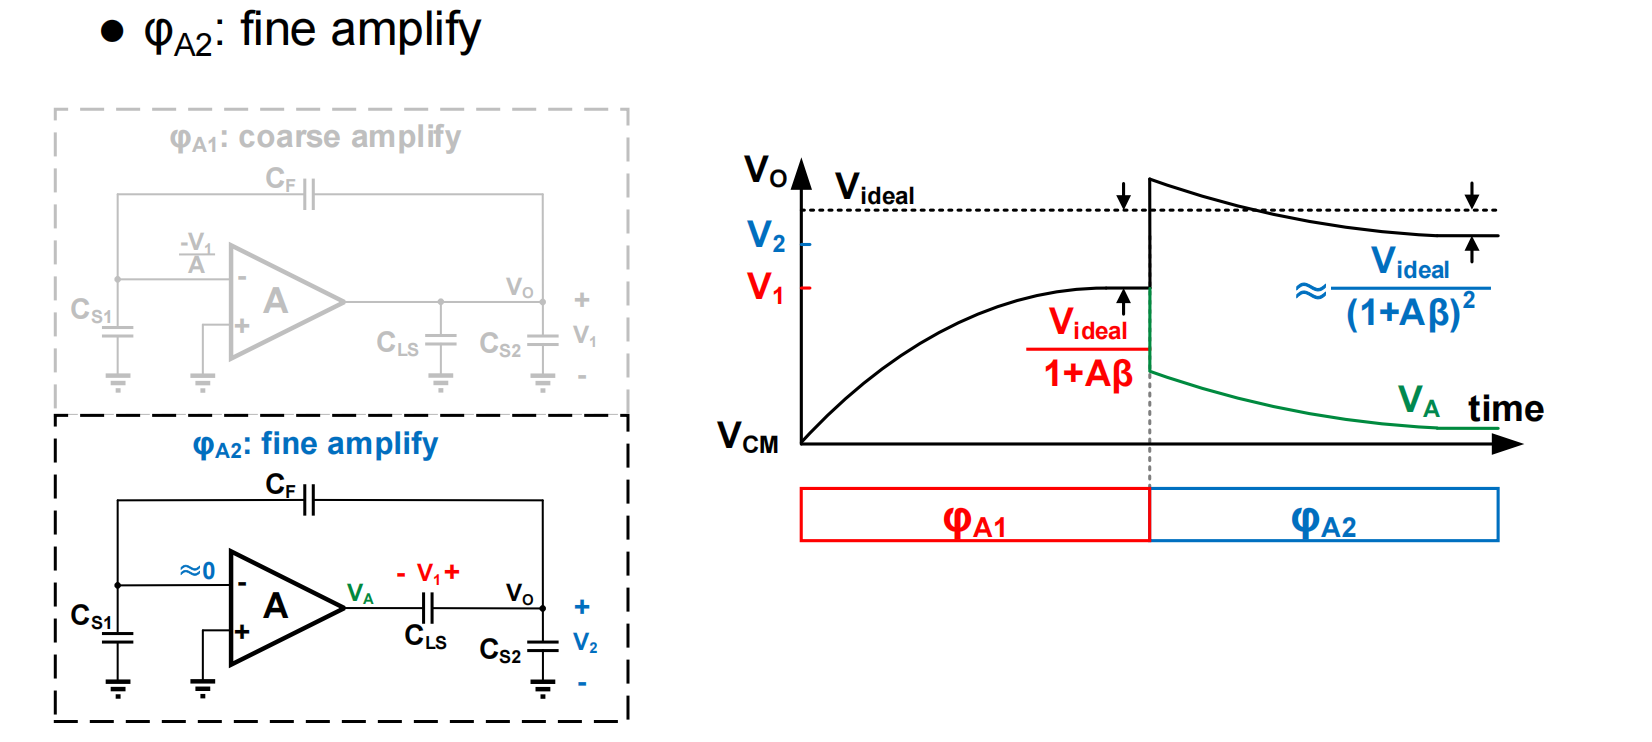
\includegraphics[width=0.48\textwidth]{doc_thesis/figs/04/CLS阶段2.png}}
\caption{CLS图示}
\label{fig:CLS图示}
\end{figure}


\subsubsection{CLS变化}

文献中CLS已形成多种变体：Two-phase CLS首先验证了相关移位在SC链路中的误差抑制可行性\cite{essam2010twophasecls}；
Averaging-CLS在流水线ADC中进一步通过相关误差平均化改善有限增益影响，
实现15-bit、22.5\,MS/s、74\,dB SNDR（90\,nm）\cite{hung2016averagingcls}；
Ping-Pong CLS将交替工作OTA与相关移位结合，提升低压动态放大效率\cite{liu2020pingpongcls}；
CR-CLS则把电平移位嵌入电荷重分配过程，使CLS从局部技巧扩展为前端放大与系统读出协同模块\cite{li2024crcls}。


\subsubsection{CLS应用}

在离散时间MASH $\Delta\Sigma$ ADC中，CLS与FIA结合可在1.2\,V供电、2.87\,$\mu$W功耗下实现94.0\,dB SNDR，
体现了微瓦级高精度前端的可实现性\cite{hu2022mashcls,meng2023jssc_mash}。
在湿度传感Zoom CDC中，CR-CLS FIA相较常规CLS-FIA在宽温和极端工艺角下可实现至少13.5\,dB开环增益提升，
并支撑0.39\,mm$^2$系统的精度与能效折中\cite{li2024crcls}。
此外，IEEE近期工作已将相关电平移位思想扩展到连续时间噪声整形SAR架构，
说明CLS正从动态放大器增益增强手段演进为跨架构低压线性化方法\cite{ye202518}。

\subsection{本研究的目的与定位}

综合已有研究可以看出，
动态放大器路线的核心矛盾是“高能效”与“高鲁棒”并存：
前者依赖极简偏置与高瞬态效率，后者要求对时序、寄生和失配具备稳定容限。
本文的研究定位即围绕该矛盾展开：在低压条件下，以 LVFIA 为基础，
引入 CLS 机制改善关键误差通道，在低压条件下提高实际增益
并在系统级场景下评估其对线性、噪声和功耗的综合收益，
为后续高能效传感读出与数据转换前端提供可复用设计方法。


\section{所提出的动态放大器设计}
在已有的LVFIA动态放大器基础上，本文提出了一种基于CLS机制的动态放大器SC电路设计，
旨在提升其在低压条件下的增益和线性性能，其原理图如图\ref{fig:the_proposed_circuit}所示
其中有些具体细节将在后文进一步补充。
\begin{figure}[htbp]
    \centering
    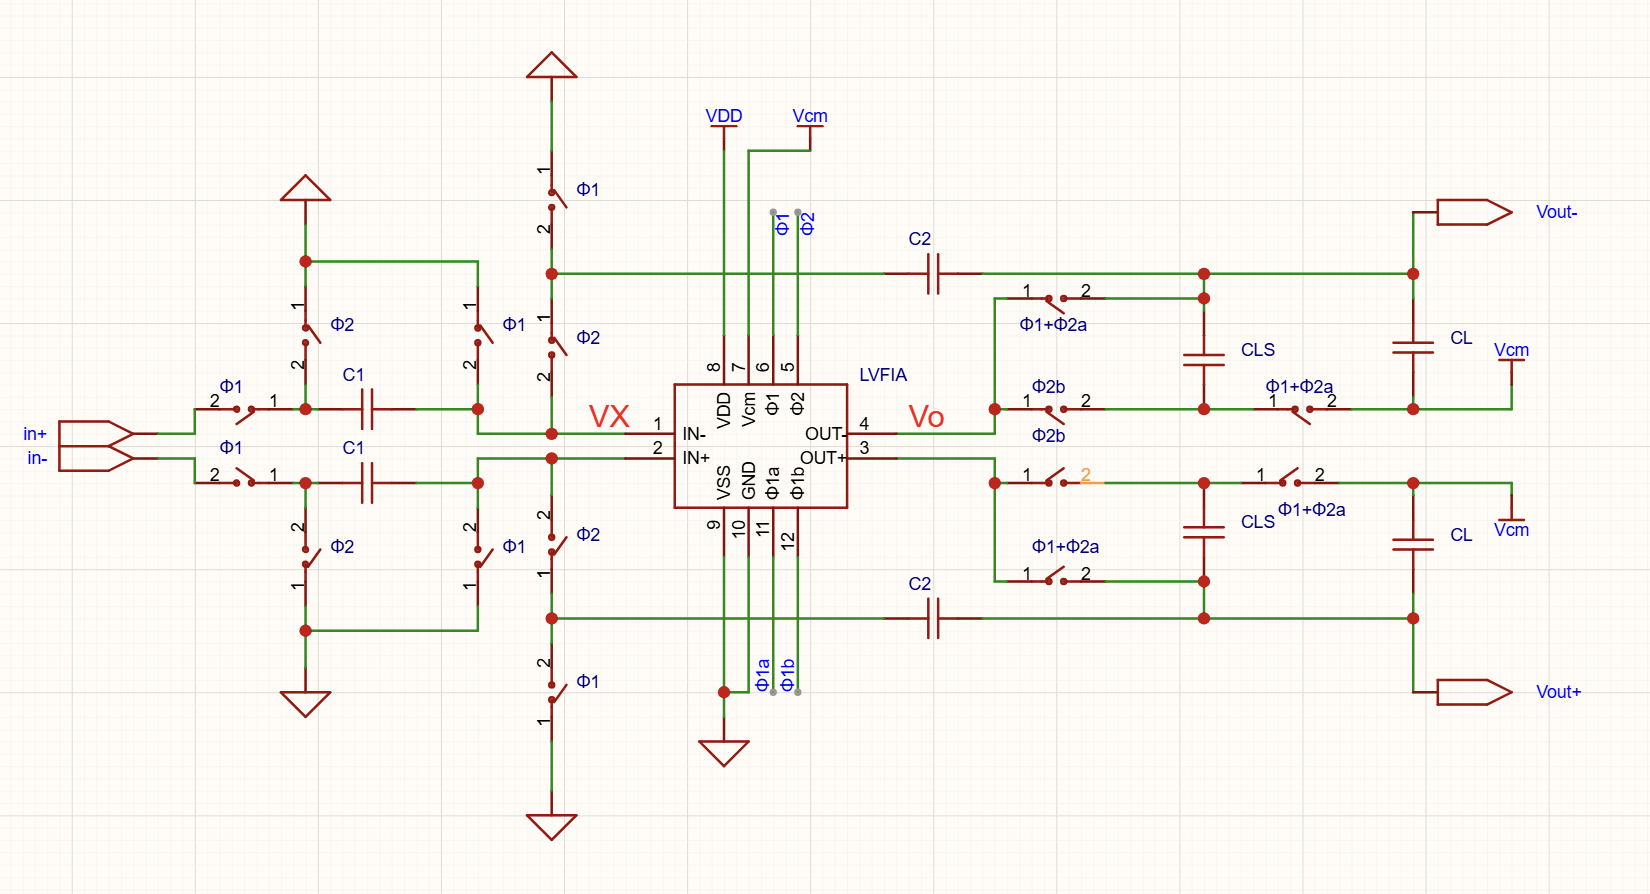
\includegraphics[width=0.8\textwidth]{doc_thesis/figs/04/the_proposed_circuit.png}
    \caption{\ptheadingfont{本论文所提出的基于LVFIA和CLS机制的动态放大器设计}}
    \label{fig:the_proposed_circuit}
\end{figure}

\subsection{电路的拓扑设计}
在电路拓扑设计方面，基于文献\cite{wu2025lvfia}LVFIA的结构，我们引入了CLS机制以实现受控的电平移位。
具体地来说，我们在基于LVFIA的积分电路的基础上增加了一个CLS电容，并且在时序上引入了一个CLS电平移位阶段，
在该阶段通过控制开关实现对输入信号的电平移位。
在复位阶段时，${\Phi_1}$=1，此时的电路连接图如图\ref{fig:reset}所示，
此时输入信号被采样到采样电容上，同时LVFIA也进行复位状态。
在放大阶段时，${\Phi_1}$=0，${\Phi_2}$=1，${\Phi_{2a}}$=1，
此时输入信号通过采样开关电容${C_1}$接入LVFIA，
同时CLS电容接入LVFIA输出端，此时${C_{CLS}}$和电容${C_L}$并联，输出电压储存到
${C_{CLS}}$和电容${C_L}$上，电路连接图如图\ref{fig:初步放大}所示。
\par
前面的两个阶段的电路拓扑和基本原理和已有的基于动态放大器的SC电路相同，
对于本文的CLS设计来说，其创新之处在于引入了电平移位阶段，通过信号${\Phi_{2b}}$控制。
在电平移位阶段，${\Phi_2}$=1，${\Phi_{2a}}$=1，${\Phi_{2b}}$=1，电路连接关系如图
\ref{fig:电平移位}所示，此时CLS电容${C_{CLS}}$串联接入输出端。以正向输出端为例，
CLS电容${C_{CLS}}$串联接入LVFIA的正相输出端和整体电路的正相输出端，且整体电路的正相输出端
电平高于LVFIA的正相输出端，这导致接入的一瞬间LVFIA的正相输出端电平被拉低，
重新启动了LVFIA的放大过程，从而提升了整体积分电路的增益。

\begin{figure}[htbp]
    \centering
    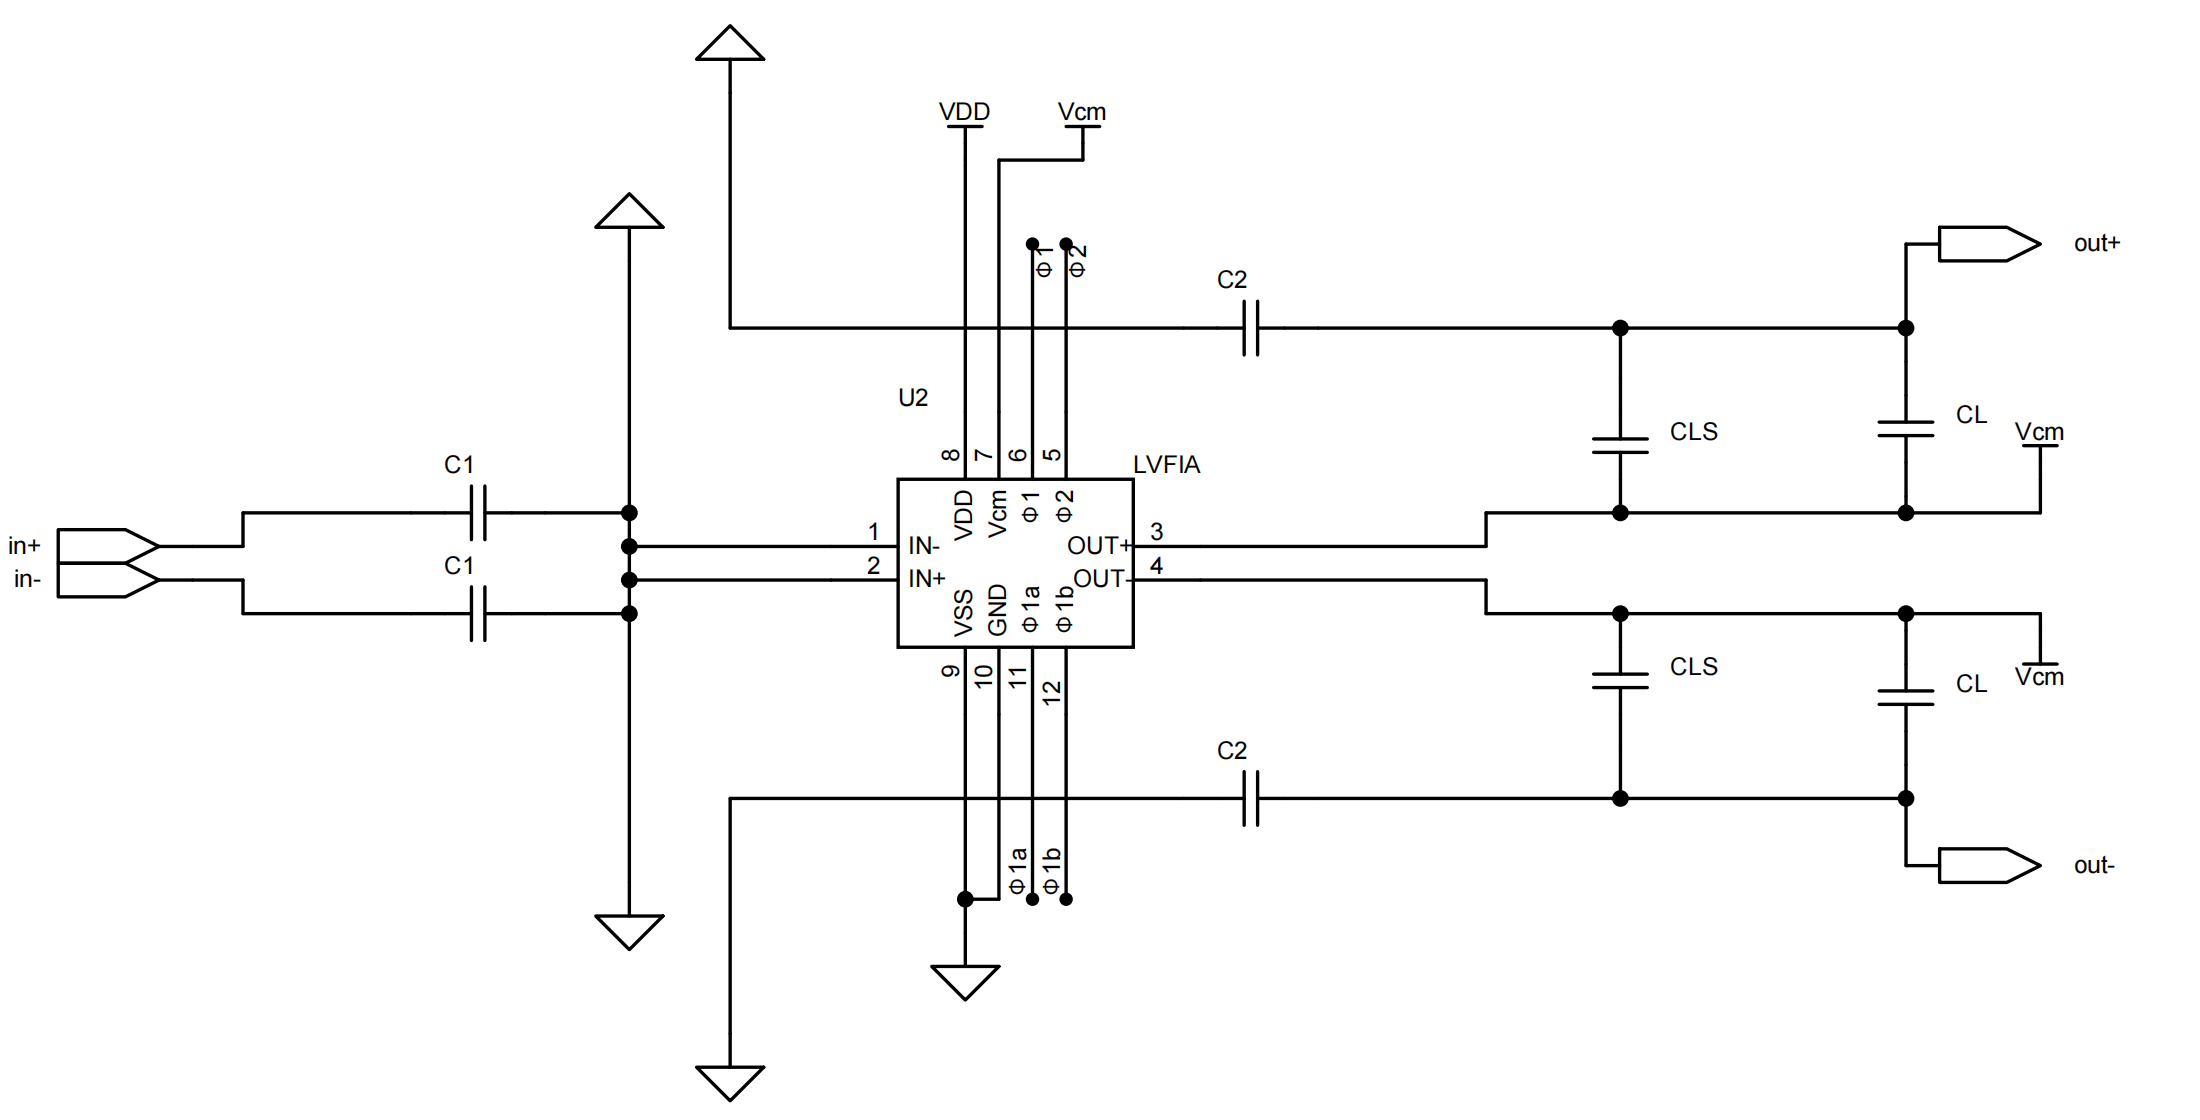
\includegraphics[width=0.8\textwidth]{doc_thesis/figs/04/复位.png}
    \caption{\ptheadingfont{复位时的电路连接关系}}
    \label{fig:reset}
\end{figure}

\begin{figure}[htbp]
    \centering
    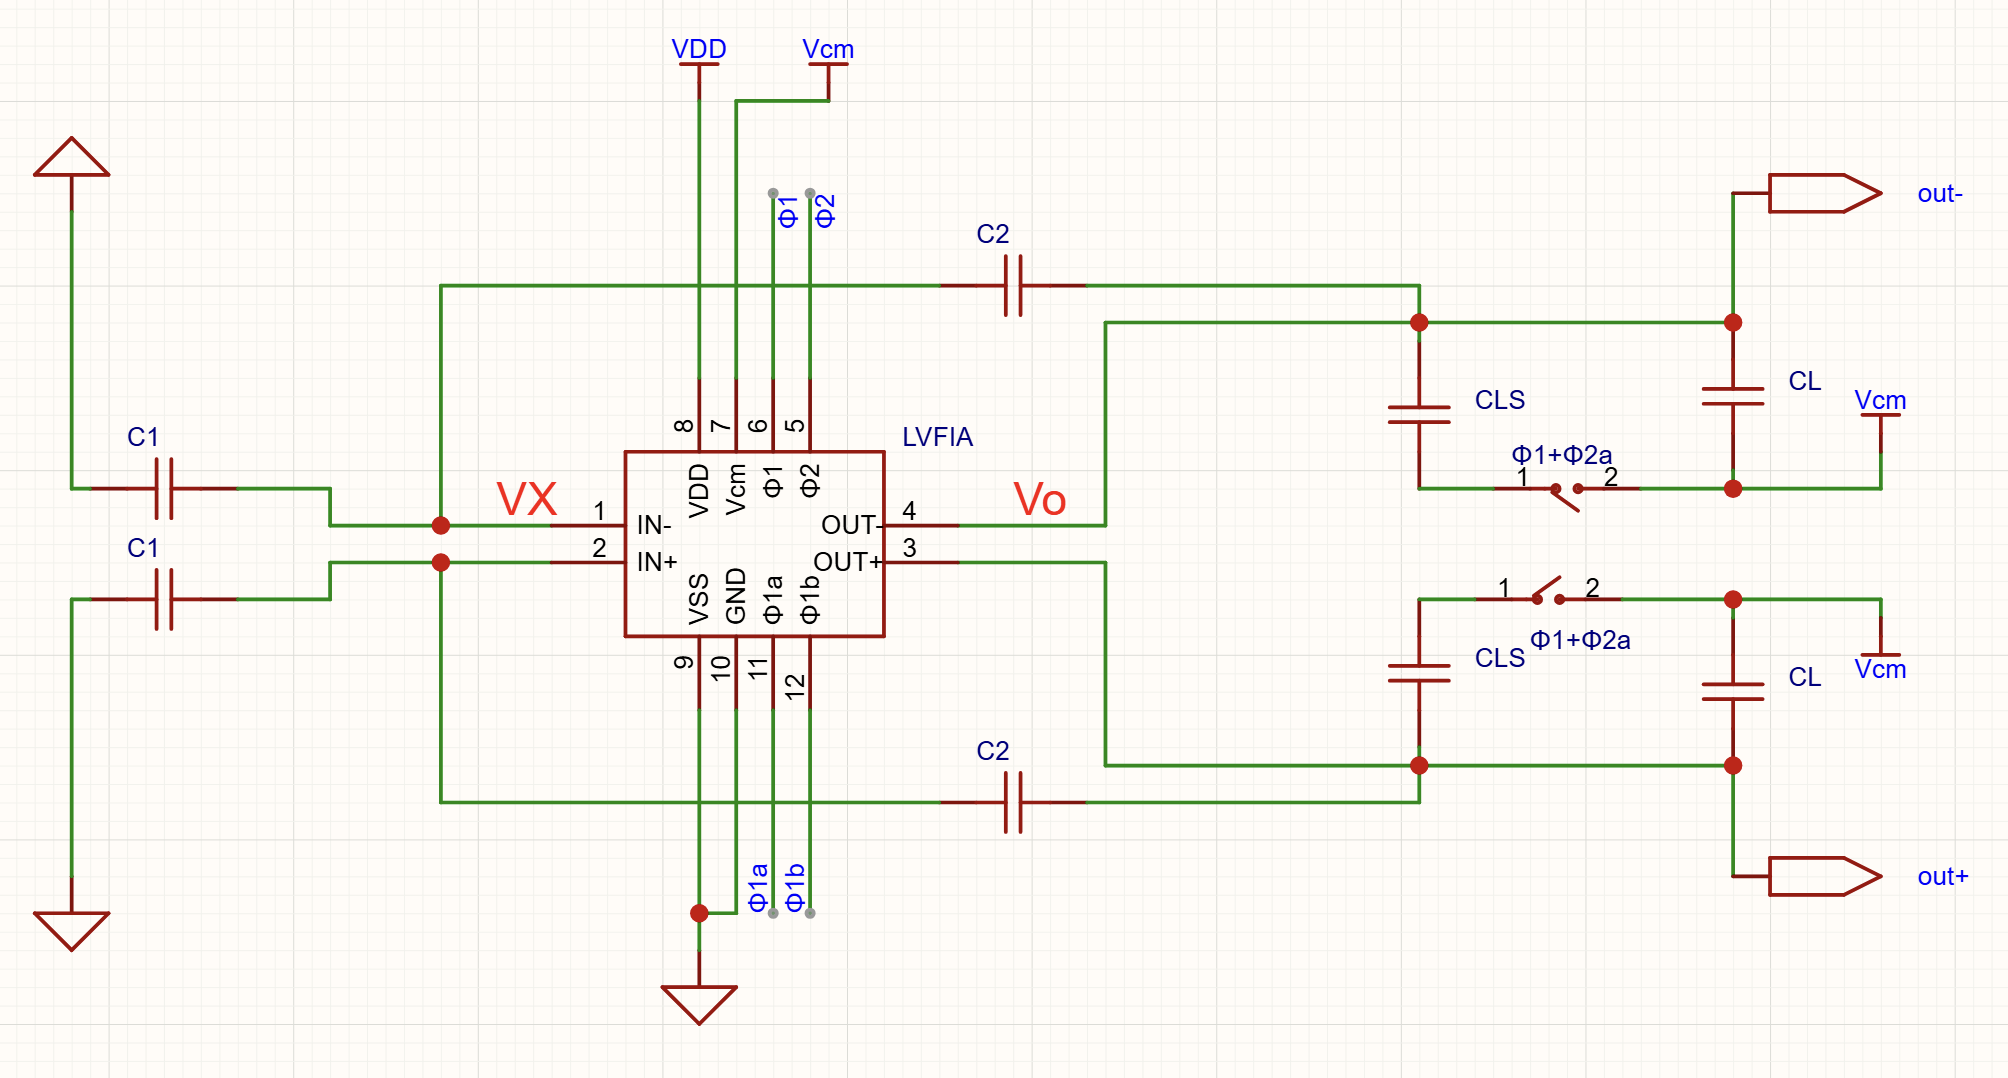
\includegraphics[width=0.8\textwidth]{doc_thesis/figs/04/初步放大.png}
    \caption{\ptheadingfont{初步放大时的电路连接关系}}
    \label{fig:初步放大}
\end{figure}

\begin{figure}[htbp]
    \centering
    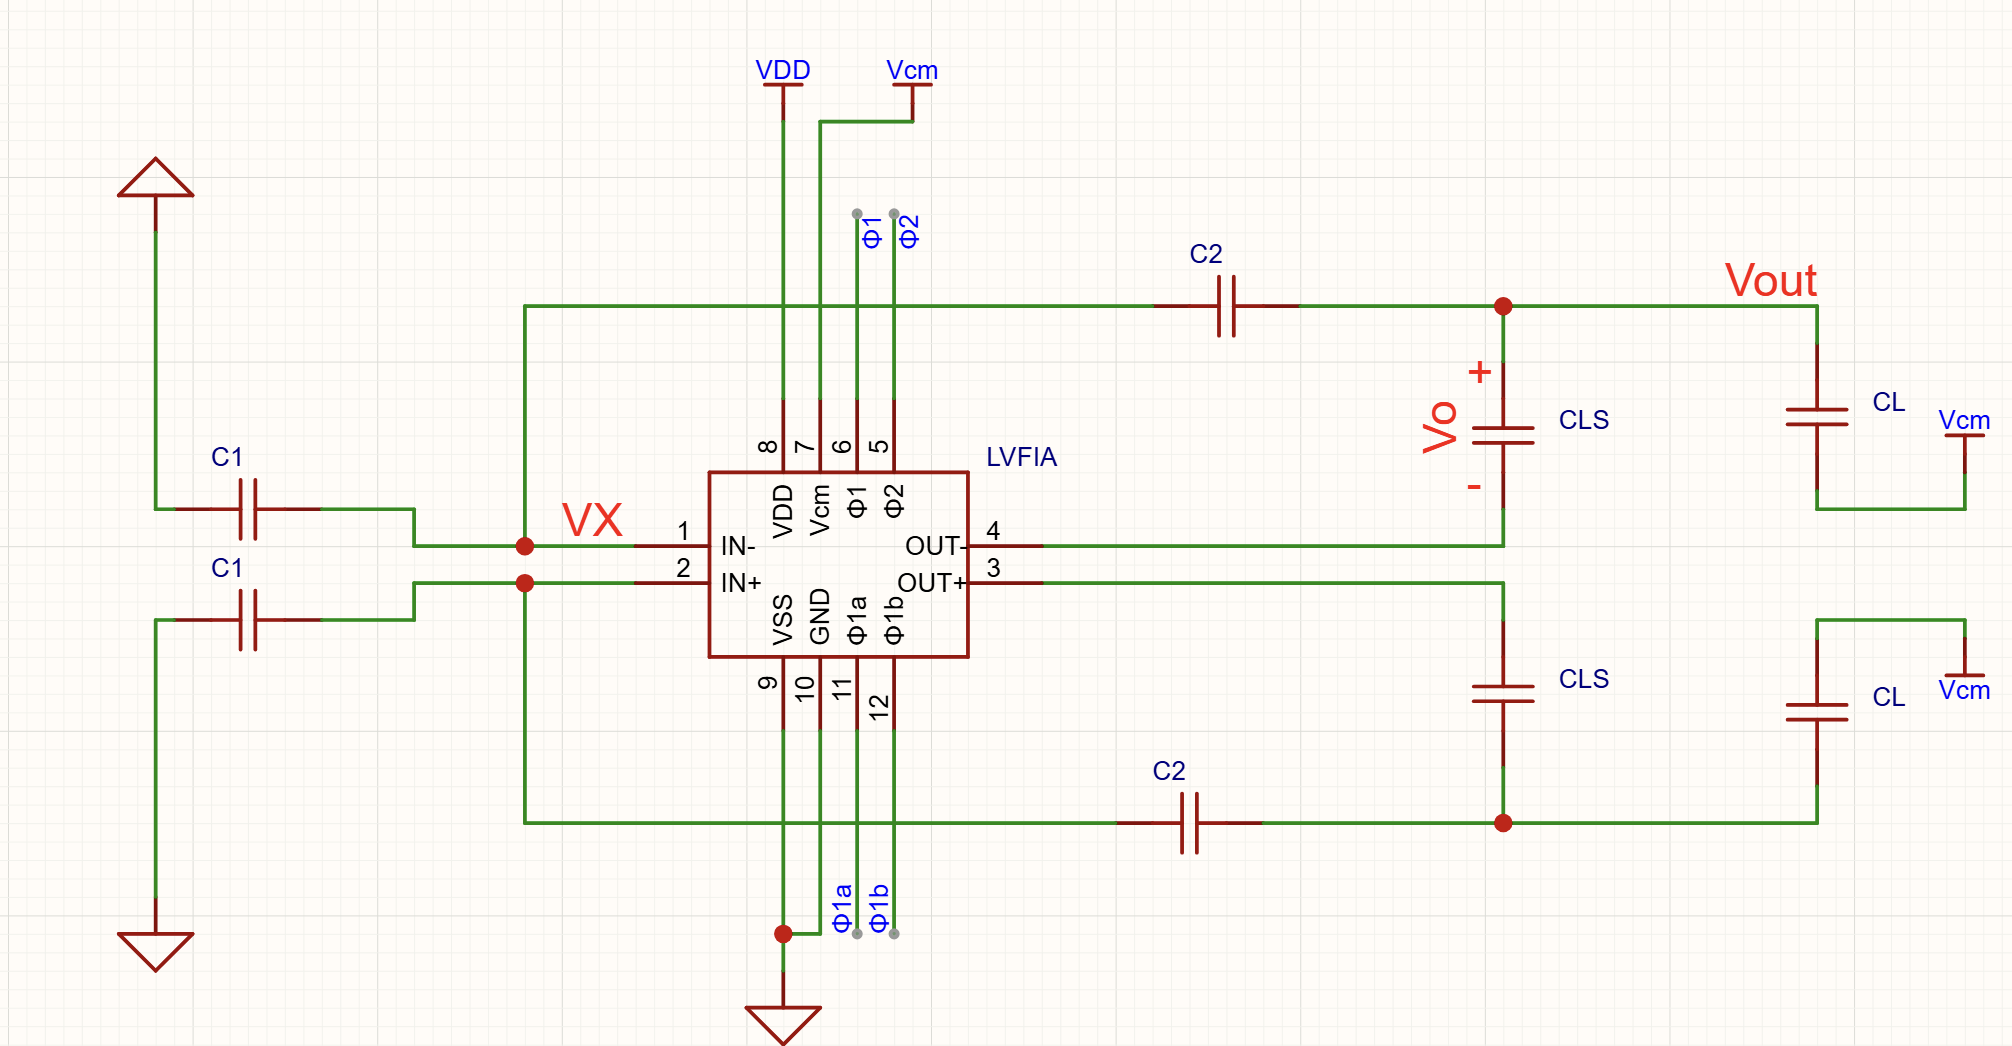
\includegraphics[width=0.8\textwidth]{doc_thesis/figs/04/电平移位.png}
    \caption{\ptheadingfont{电平移位时的电路连接关系}}
    \label{fig:电平移位}
\end{figure}

\subsection{增益提升}
下面进行具体分析为什么串联的电平移位电容可以增加积分电路的增益。
对于存在反馈电容${C_2}$的开关电容积分器（Switched-Capacitor, SC）来说，考虑到电容
${C_2}$跨接在LVFIA的反相输入端和输出端，LVFIA的正相和反相输入端之间可以认为是断路
（LVFIA的输入端接MOS管栅级，没有电流通过）但是并不短路（LVFIA增益有限，无法像理想运放那样认为是“虚短”）。
由于输入端没有电流，所以输出端给电容${C_2}$提供的电荷只能来自于输入端的电容${C_1}$,
因此可以认为输入端的电容${C_1}$向输出端的电容${C_2}$转移电荷越多，
${C_1}$两端电压差${V_{C_1}}$越小，输出端的电压${V_{C_2}}$越大。
为简化分析，假设LVFIA具有固定直流电压增益A（实际上LVFIA的增益会随时间变化，在放大阶段的最后
达到最大），LVFIA单端输入电压为${V_X}$，输出电压为${V_o}$，则可以得到如下关系：
\begin{equation}
    {V_X} = -\frac{V_o}{A} 
\end{equation}
因此减小${V_X}$的绝对值可以通过减小${V_o}$的绝对值来实现，
而电平移位过程中，由于${C_{CLS}}$串联在输入端，此时的${V_X}$表达式为
\begin{equation}
    {V_X} = -\frac{V_{out}-V_o}{A} 
\end{equation}
通过电平移位操作显著减小了${V_X}$的绝对值，使得采样电容${C_1}$能够更有效地向
${C_2}$以及输出端${C_L}$转移电荷，从而提升了整体积分电路的增益。
\par
进行定量分析，对于没有引入CLS的SC放大器，如果反馈回路的电容比为${\frac{C_1}{C_2} }$，
则其增益为
\begin{equation}
    \frac{V_o}{V_{in}} = \frac{C_1}{C_2}\cdot\frac{1}{1+\frac{1}{T} }
\end{equation}
其中T为环路增益，也即
\begin{equation}
    T = \frac{C_2}{C_1}\cdot A_{lvfia}
\end{equation}
而在引入了CLS之后，此时的闭环SC放大器增益约为
\begin{equation}
    \frac{V_{out}}{V_{in}}
    =-\frac{C_1}{C_2}\cdot
    \frac{1}{1+\frac{1}{T_{cls}} }
\end{equation}
其中$T_{cls}$为引入CLS之后的环路增益，根据理论分析，满足
\begin{equation}
    T_{cls} \approx T^2
\end{equation}
可见引入CLS之后等效的环路增益明显提升，继而减小了SC放大器增益公式中的误差项，
使得整体增益更接近于理想的电容比值$\frac{C_1}{C_2}$。

\subsection{线性度提升}
同时，由于电平移位操作减小了输入端的电压差，电路的整体输出不是和LVFIA输出端直接相连，
也就是说，原本SC积分器的输出端电压${V_{C_L}}$直接由LVFIA的输出电压${V_o}$决定，
而引入电平移位后，输出端电压${V_{C_L}}$由电平移位后的电压${V_{out}}$决定，且有
\begin{equation}
    {V_{C_L}} = {V_o} + {V_{C_{CLS}}}
\end{equation}
在相同的输出电压下，电平移位操作使得LVFIA的输入端电压绝对值${V_X}$以及
输出电压${V_o}$降低，从而减小了
LVFIA的非线性失真对整体输出的影响，
提升了整体电路的线性度。

\subsection{设计变体}
通过上述分析，我们得知，引入CLS电容可以在电平移位阶段通过CLS电容的串联接入
降低LVFIA的输入和输出电压，增加输入电容${C_1}$的放电量，提升整体电路的增益和线性度。
那么由此产生的一个比较自然的想法是，是否可以通过增加更多的CLS电容来进一步提升增益和线性度。
例如在电平移位阶段时，使用两个移位电容${C_{CLS1}}$和${C_{CLS2}}$串联接入输出端，
能够进一步降低LVFIA的输入和输出电压，从而预期能够进一步提升增益和线性度。
不过通过理论分析和仿真验证我们发现，增加CLS电容带来的增益提升存在边际效应递减。





\section{电路设计和测试结果}

\subsection{工艺库和参数设置}
本论文的电路设计和仿真基于TSMC 130nm工艺库。对于LVFIA，其包含了所有输入输出端口的电路原理图
以及对应的元件模型如图\ref{fig:LVFIA的原理图和器件模型}所示，作为一个典型的基于开关电容的
浮动反相动态放大器，其核心结构包含了一对PMOS和NMOS晶体管，
输入端接在两者的栅极，输出端分别接在两者的漏极；
以及一个储能电容${C_{RES}}$接在两者的源极，复位阶段由电源对储能电容充电，放大阶段时储能电容放电偏置晶体管。
此外，LVFIA的输入端配置有偏置电容${C_c}$，在复位和自归零阶段能够定义和储存
NMOS和PMOS的偏置电压，确保放大阶段的稳定工作点。LVFIA的负载电容${C_L}$
则在LVFIA片外配置。
\par
上述提到的所有元件均在TSMC 130nm工艺库中完成，其中PMOS和NMOS晶体管模型为
pmos1v-mis和nmos1v-mis，该模型为亚1V工艺下的晶体管模型，能够反映出晶体管在低压条件下的性能表现；
储能电容${C_{RES}}$和偏置电容${C_c}$则使用了工艺库中的NMOS电容模型nmos1vcap。
此外，电路中的所有开关均由NMOS晶体管实现，使用模型为nmos1v-mis。
作为数字信号，其高电平为1V时开关导通，低电平为0V时开关截止。
LVFIA的元件参数设置如下表\ref{tab:参数设置}所示。

\begin{table}[htbp]
    \centering
    \caption{\ptheadingfont{LVFIA的参数设置}}
    \label{tab:CLS参数设置}
    \begin{tabular}{|c|c|}
        \hline
         参数名 & 值 \\
        \hline
        偏置电容${C_c}$ & 5pF  \\
        \hline
        储能电容${C_{RES}}$ & 25pF  \\
        \hline
    \end{tabular}
\end{table}





对于包含LVFIA的完整CLS开关电容放大器，其包含了上述LVFIA的结构，
同时在输入端包含了输入电容${C_1}$，输出端包含CLS电容${C_{CLS}}$以及负载电容${C_L}$。
这一部分的参数设置如下表所示：
\begin{table}[htbp]
    \centering
    \caption{\ptheadingfont{CLS开关电容放大器的参数设置}}
    \label{tab:参数设置}
    \begin{tabular}{|c|c|}
        \hline
         参数名 & 值 \\
        \hline
        输入电容${C_1}$ & 1pF  \\
        \hline
        反馈电容${C_2}$ & 200fF  \\
        \hline
        移位电容${C_{CLS}}$ & 500fF  \\
        \hline
        负载电容${C_L}$ & 10fF  \\
        \hline
    \end{tabular}
\end{table}

\begin{figure}[htbp]
\centering
\subfigure[LVFIA的原理图]{
		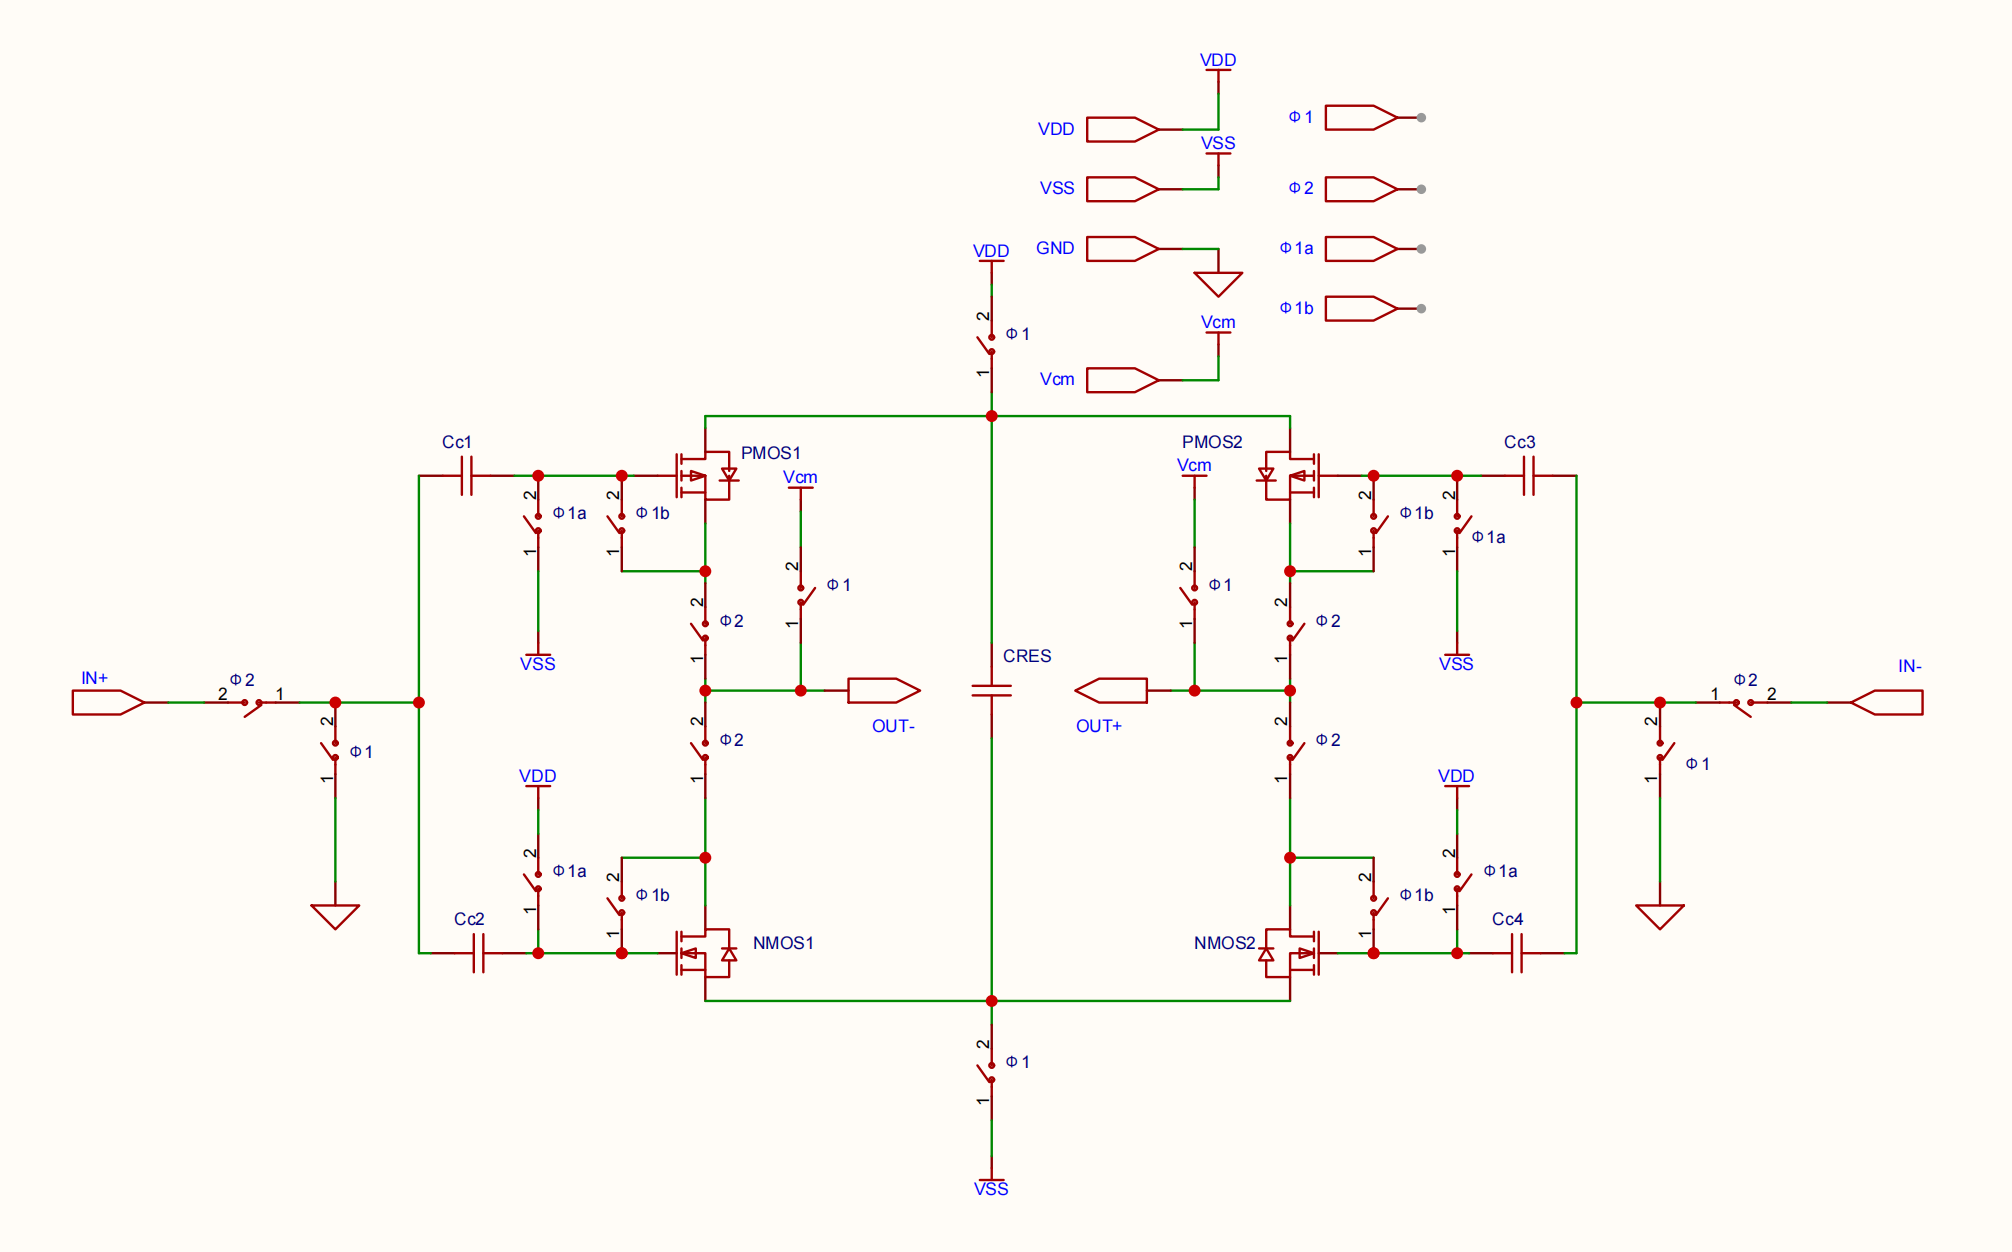
\includegraphics[width=0.48\textwidth]{doc_thesis/figs/04/LVFIA_schematic.png}}
\hfill
\subfigure[LVFIA的器件模型]{
		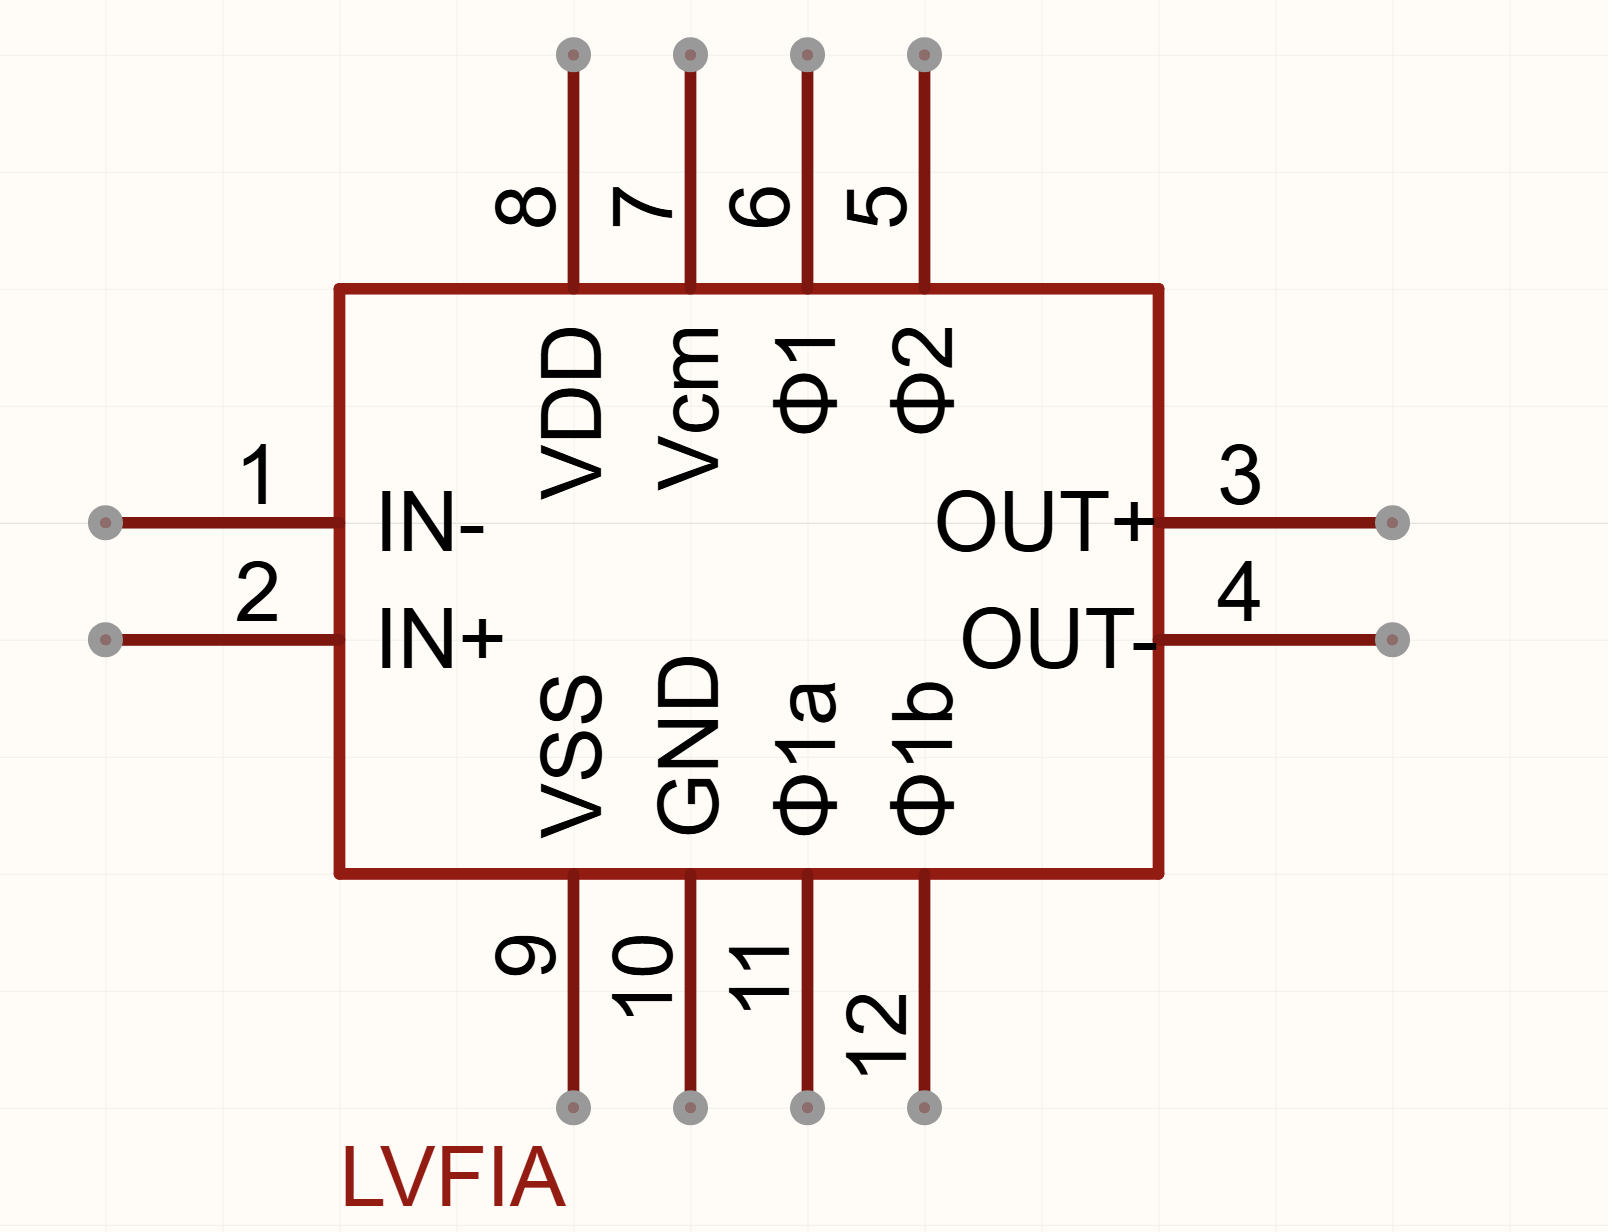
\includegraphics[width=0.48\textwidth]{doc_thesis/figs/04/LVFIA_model.png}}
\caption{LVFIA的原理图和器件模型}
\label{fig:LVFIA的原理图和器件模型}
\end{figure}

\begin{figure}[htbp]
    \centering
    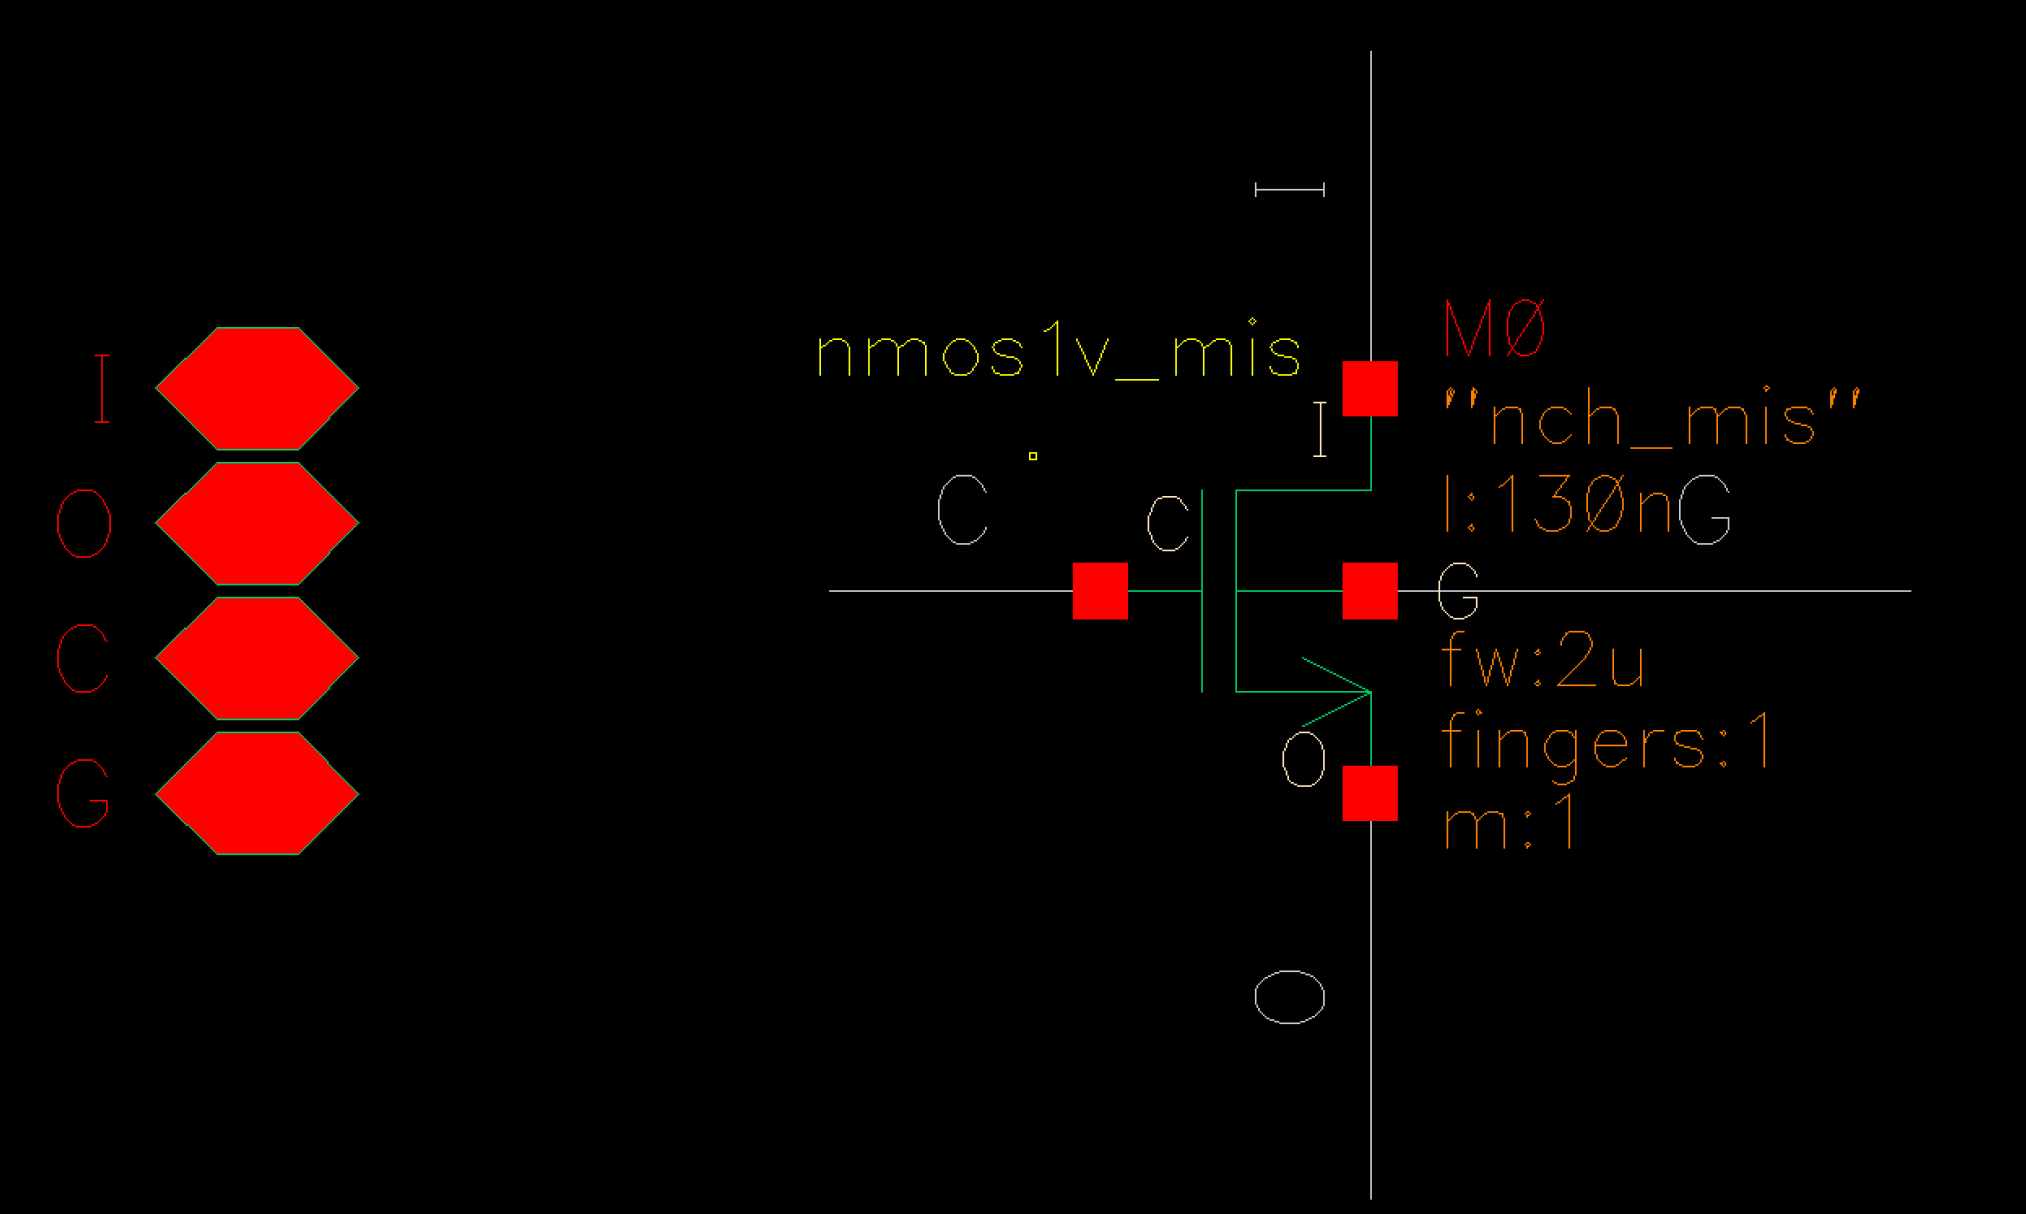
\includegraphics[width=0.8\textwidth]{doc_thesis/figs/04/模拟开关.png}
    \caption{\ptheadingfont{在Cadence中基于nmos1v-mis模型设计的模拟开关
    端口C：控制信号接入；端口G：接地；端口I、O：输入输出端口}}
    \label{fig:模拟开关}
\end{figure}


\subsection{电路增益}
CLS技术带来的最关键的性能提升即为增益提升，在Cadence仿真环境下，我们对引入CLS机制前后的
动态放大器电路进行了仿真测试，在不同PVT条件下对电路的增益、线性度等性能指标进行了评估。
需要注意的是，在引入CLS机制后，可以将电平移位阶段的LVFIA和CLS电容作为一个整体
的动态放大器单元，通过测量其开环增益来评估CLS带来的等效增益提升；也可以测量引入CLS
前后SC放大器的闭环增益，然后通过比对其误差的减小情况，通过公式\ref{equa:SC_amplifier_1}
和公式\ref{equa:SC_amplifier_2}来反推CLS带来的等效增益提升。

\begin{figure}[htbp]
    \centering
    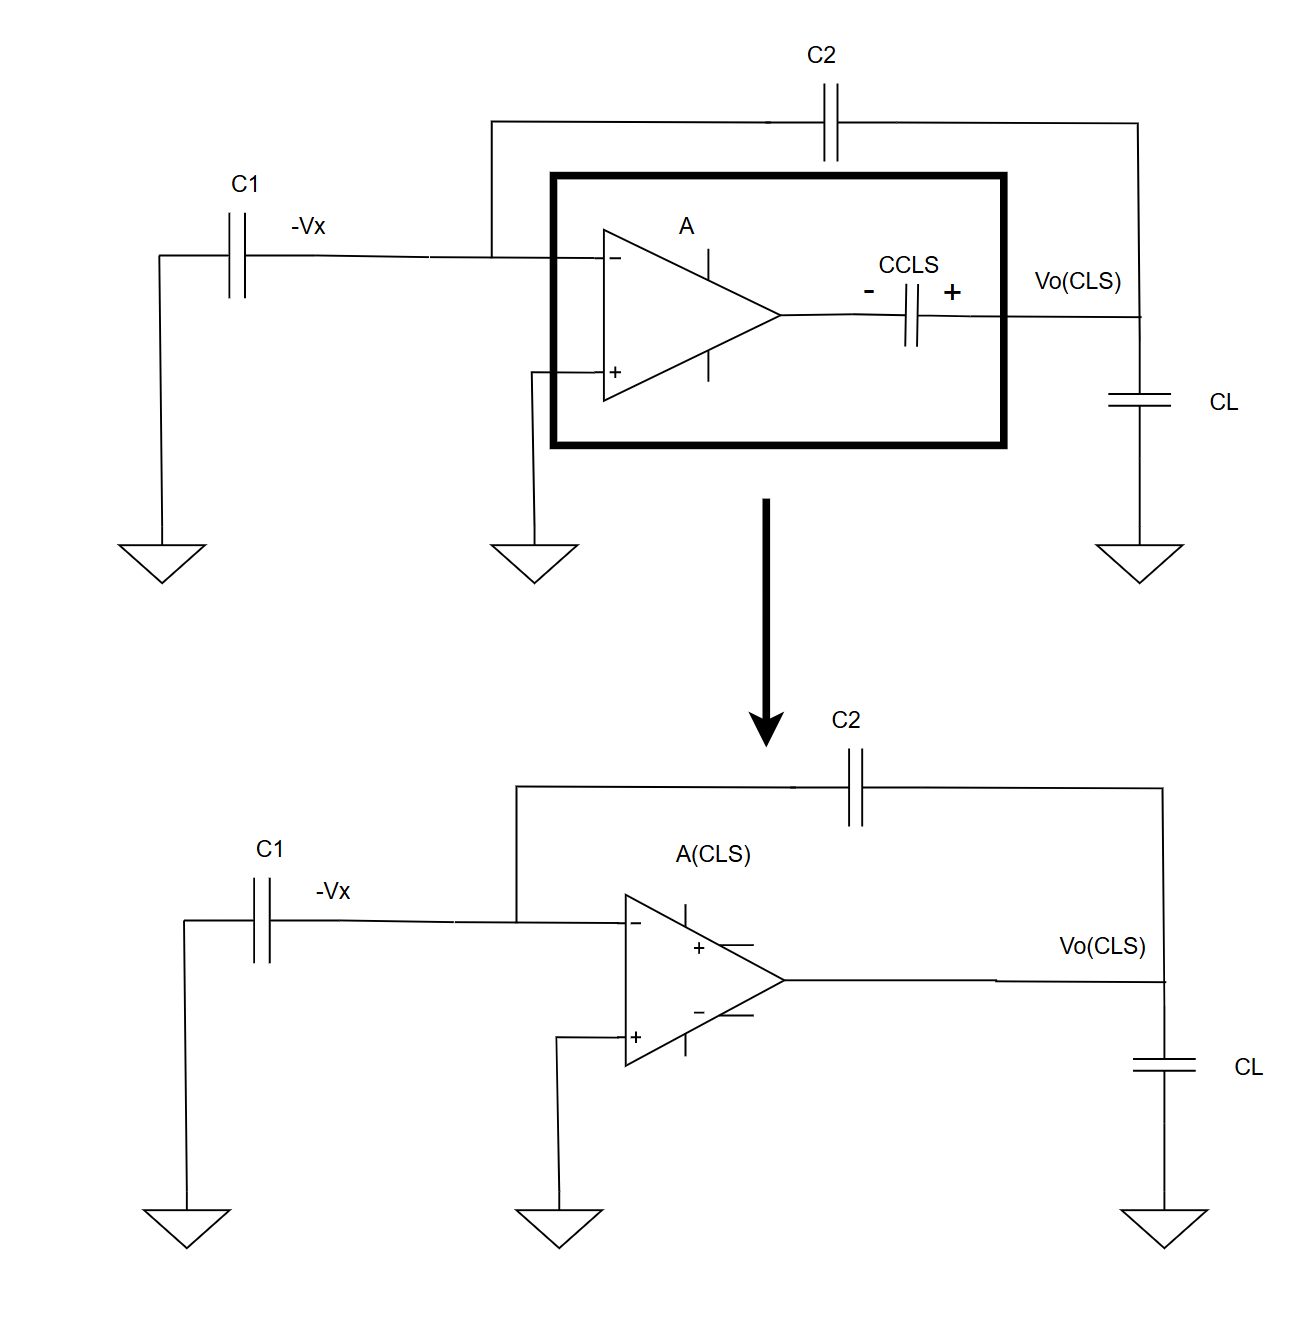
\includegraphics[width=0.8\textwidth]{doc_thesis/figs/04/应用CLS之后等效增益的计算方法.png}
    \caption{\ptheadingfont{引入CLS之后，将LVFIA和CLS电容作为一个整体来测量其增益提升}}
    \label{fig:应用CLS之后等效增益的测量方法}
\end{figure}


\begin{table}[htbp]
    \centering
    \caption{\ptheadingfont{不同PVT条件下的CLS电路开环增益}}
    \label{tab:CLS电路开环增益}
    \begin{tabular}{|c|c|c|c|c|c|c|}
        \hline
         温度（单位：°C）/电压（单位：V） & 0.7 & 0.65 & 0.6 & 0.55 &0.5 &0.45 \\
        \hline
        -40 & 46.27 & 49.55 & 53.78 & 56.47 & 57.55 & 57.55 \\
        \hline
        25 & 43.56 & 46.50  & 49.44 & 53.13 & 55.31 & 55.31 \\
        \hline
        80 & 23.41 & 32.84 & 35.42 & 37.04 & 37.79 & 37.79 \\
        \hline
    \end{tabular}
\end{table}

\begin{table}[htbp]
    \centering
    \caption{\ptheadingfont{不同PVT条件下无CLS的LVFIA电路开环增益}}
    \label{tab:无CLS的LVFIA电路开环增益}
    \begin{tabular}{|c|c|c|c|c|c|c|}
        \hline
         温度（单位：°C）/电压（单位：V） & 0.7 & 0.65 & 0.6 & 0.55 &0.5 &0.45 \\
        \hline
        -40 & 23.65 & 25.07 & 26.16 & 26.68 & 26.68 & 26.68 \\
        \hline
        25 & 20.13 & 21.62   & 22.51 & 23.08 & 23.33 & 23.33 \\
        \hline
        80 & 12.67 & 18.85 & 20.65 & 21.97 & 22.91 & 23.45 \\
        \hline
    \end{tabular}
\end{table}

\begin{figure}[htbp]
    \centering
    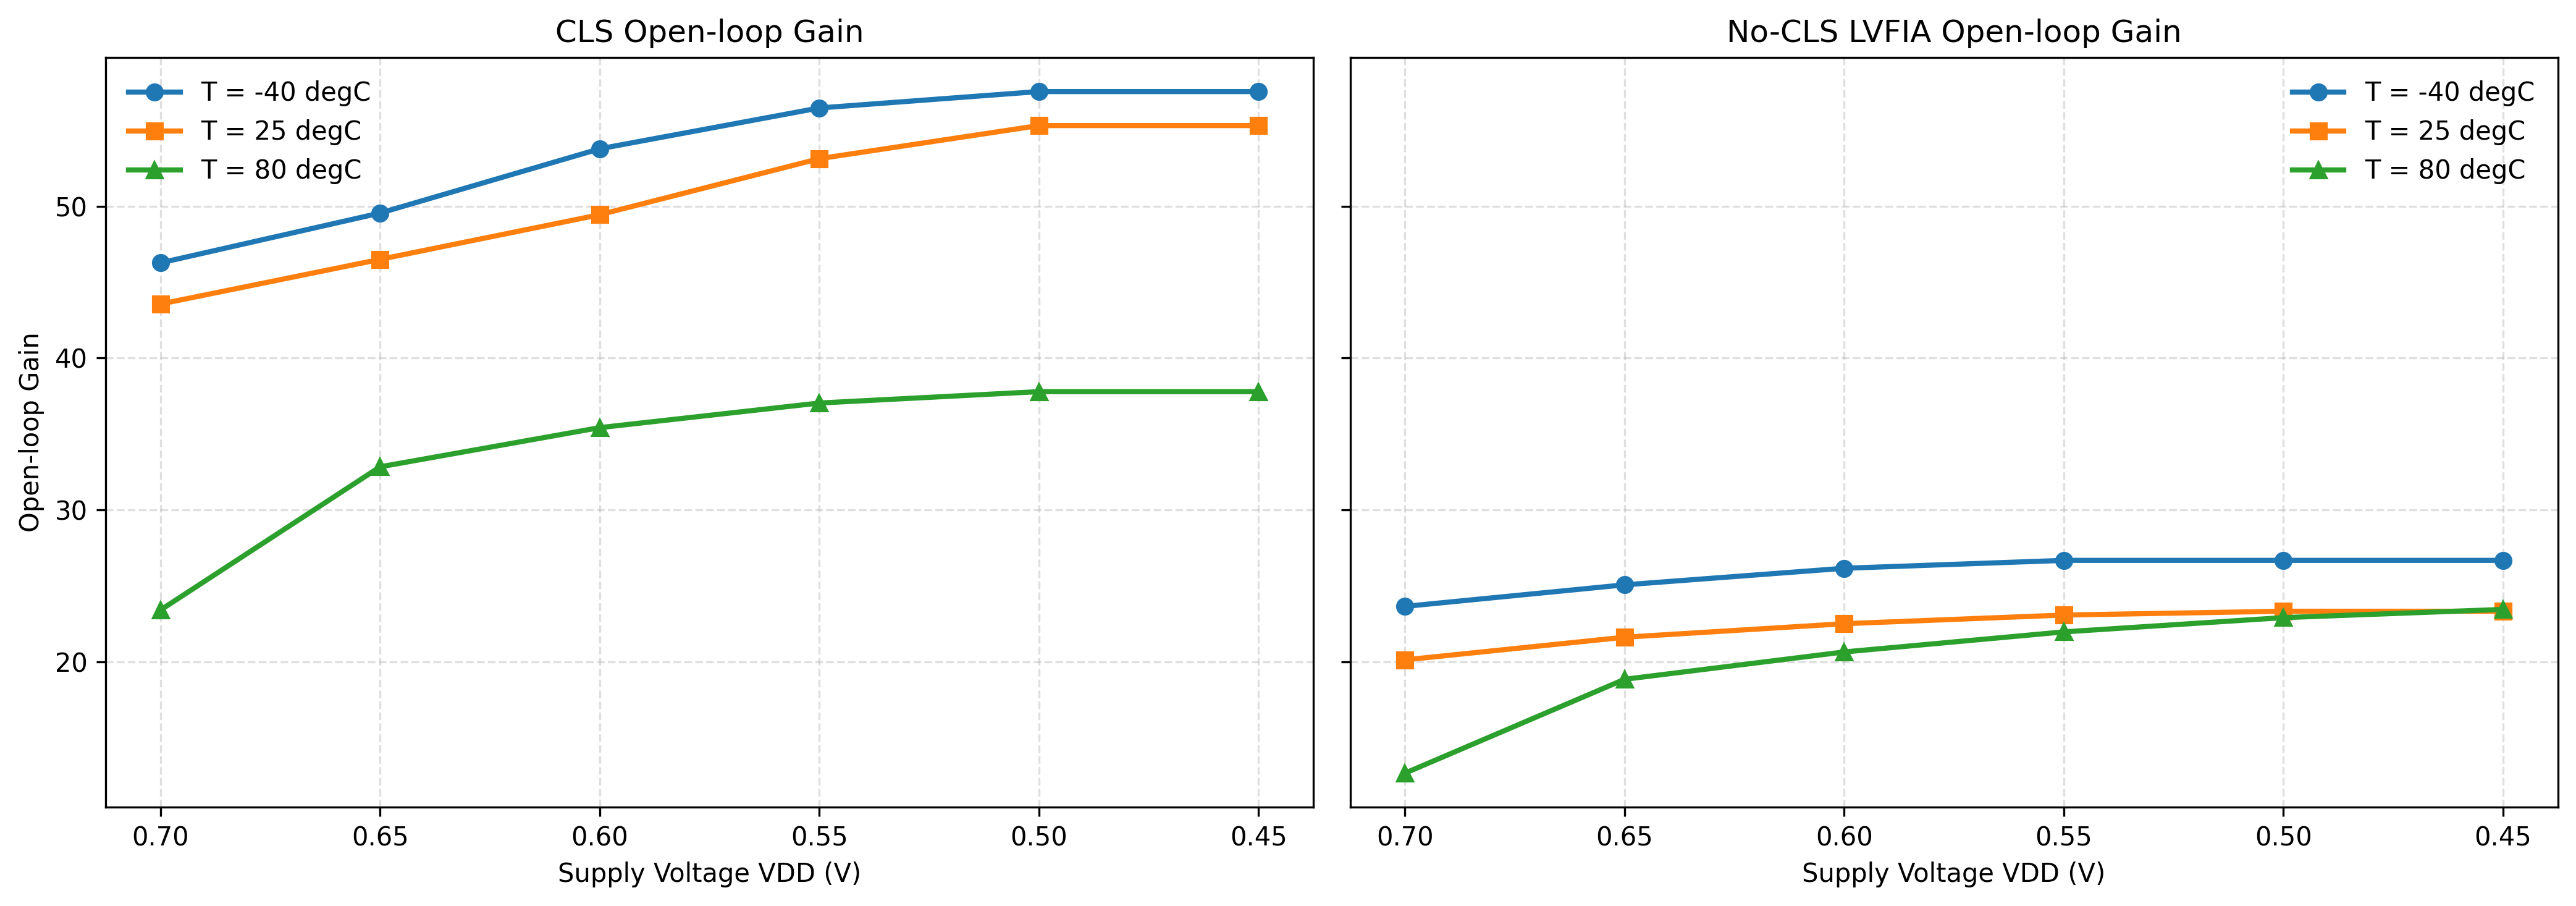
\includegraphics[width=0.8\textwidth]{doc_thesis/figs/04/pvt_open_loop_gain.png}
    \caption{\ptheadingfont{开环增益随PVT变化的趋势图}}
    \label{fig:开环增益随PVT变化的趋势图}
\end{figure}

在一般应用中，更多用到的是带有反馈电容的闭环开关电容放大器，并且该电容一般设置成可调节的，
因此我们也对引入CLS机制前后的电路闭环增益进行了测试。在25℃，电源电压$V_{DD}$=0.6V的条件下，
测试了不同反馈电容值${C_2}$下的电路增益，结果如表\ref{tab:CLS电路闭环增益}所示。
图\ref{fig:有无CLS下的瞬态响应对比}则展示了在相同条件下有无CLS机制的电路
在Cadence瞬态仿真下的响应对比，可见在初步放大阶段${\Phi_{2a}=1}$时两者增益几乎一致，
但是在电平移位阶段${\Phi_{2b}=1}$时引入CLS机制的电路增益显著提升，


\begin{table}[htbp]
    \centering
    \caption{\ptheadingfont{CLS电路闭环增益}}
    \label{tab:CLS电路闭环增益}
    \begin{tabular}{|c|c|c|c|c|c|c|}
        \hline
         有无CLS/${\frac{C_1}{C_2} }$ & 2 & 10 & 20 & 40 & 100 & 200 \\
        \hline
        有CLS & 1.99 & 8.74 & 15.12 & 24.30 & 36.06 & 42.58 \\
        \hline
        无CLS & 1.78 & 6.73  & 10.37 & 14.26 & 18.44 & 20.22 \\
        \hline
    \end{tabular}
\end{table}

\begin{figure}[htbp]
    \centering
    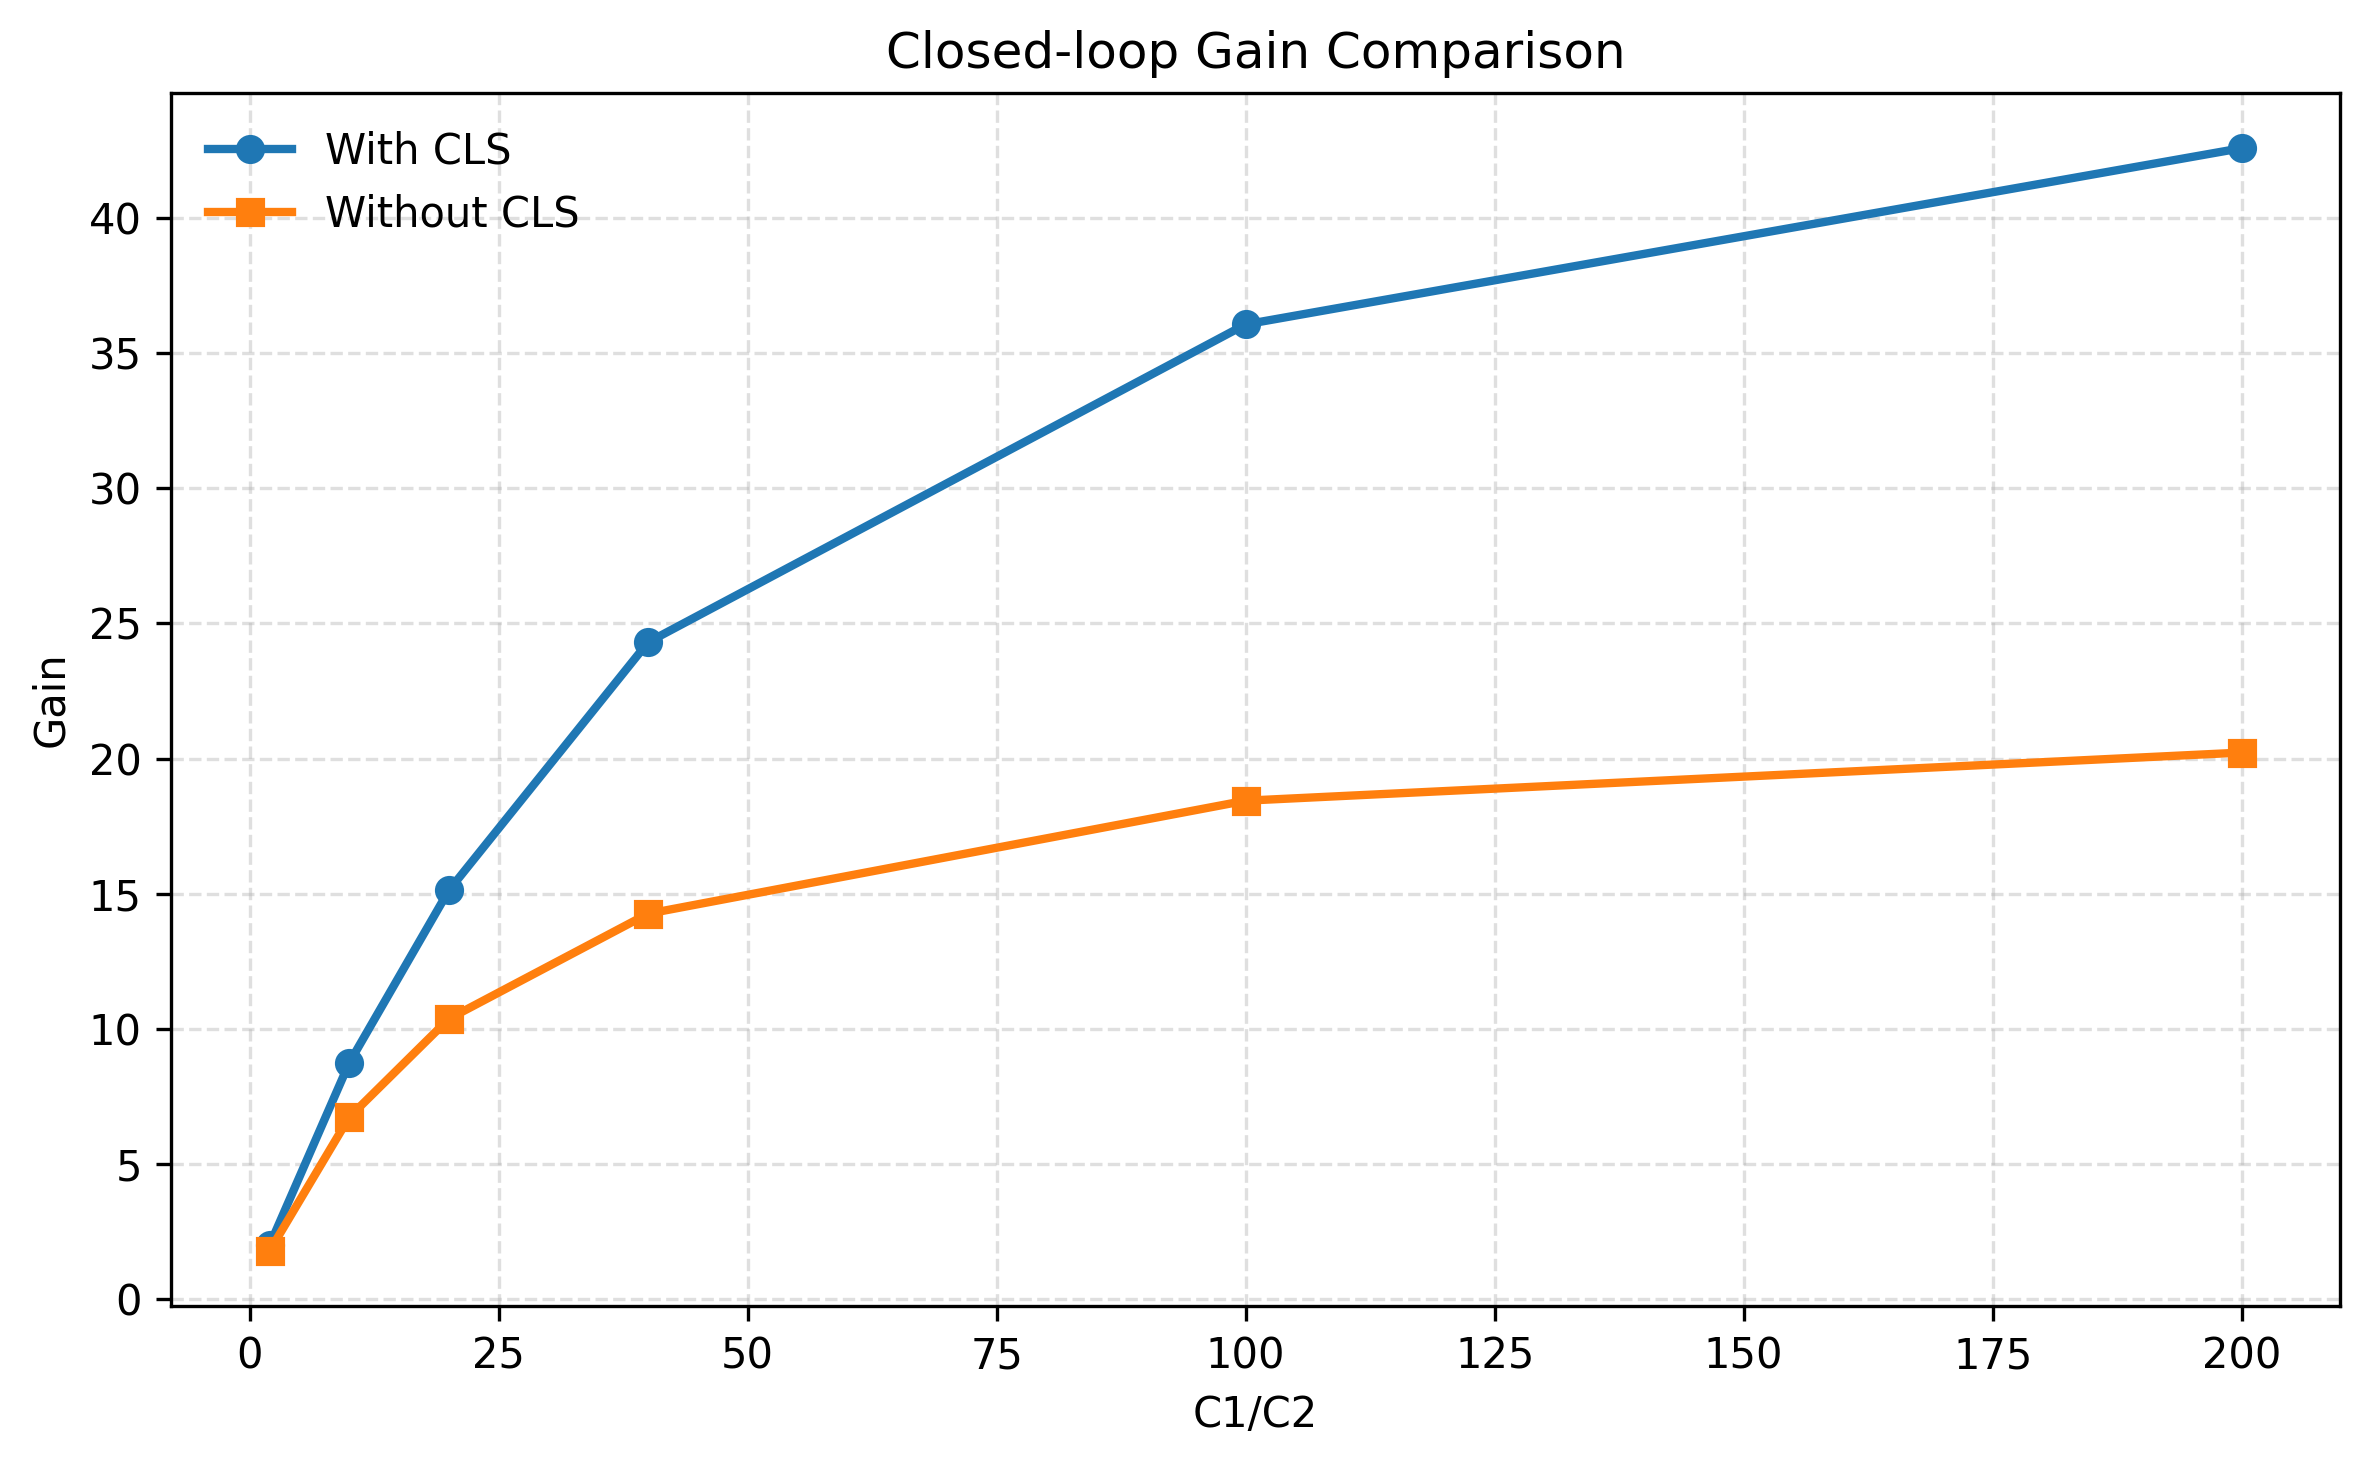
\includegraphics[width=0.8\textwidth]{doc_thesis/figs/04/cls_closed_loop_gain.png}
    \caption{\ptheadingfont{闭环增益随C1/C2变化的趋势图}}
    \label{fig:闭环增益随C1/C2变化的趋势图}
\end{figure}

\begin{figure}[htbp]
    \centering
    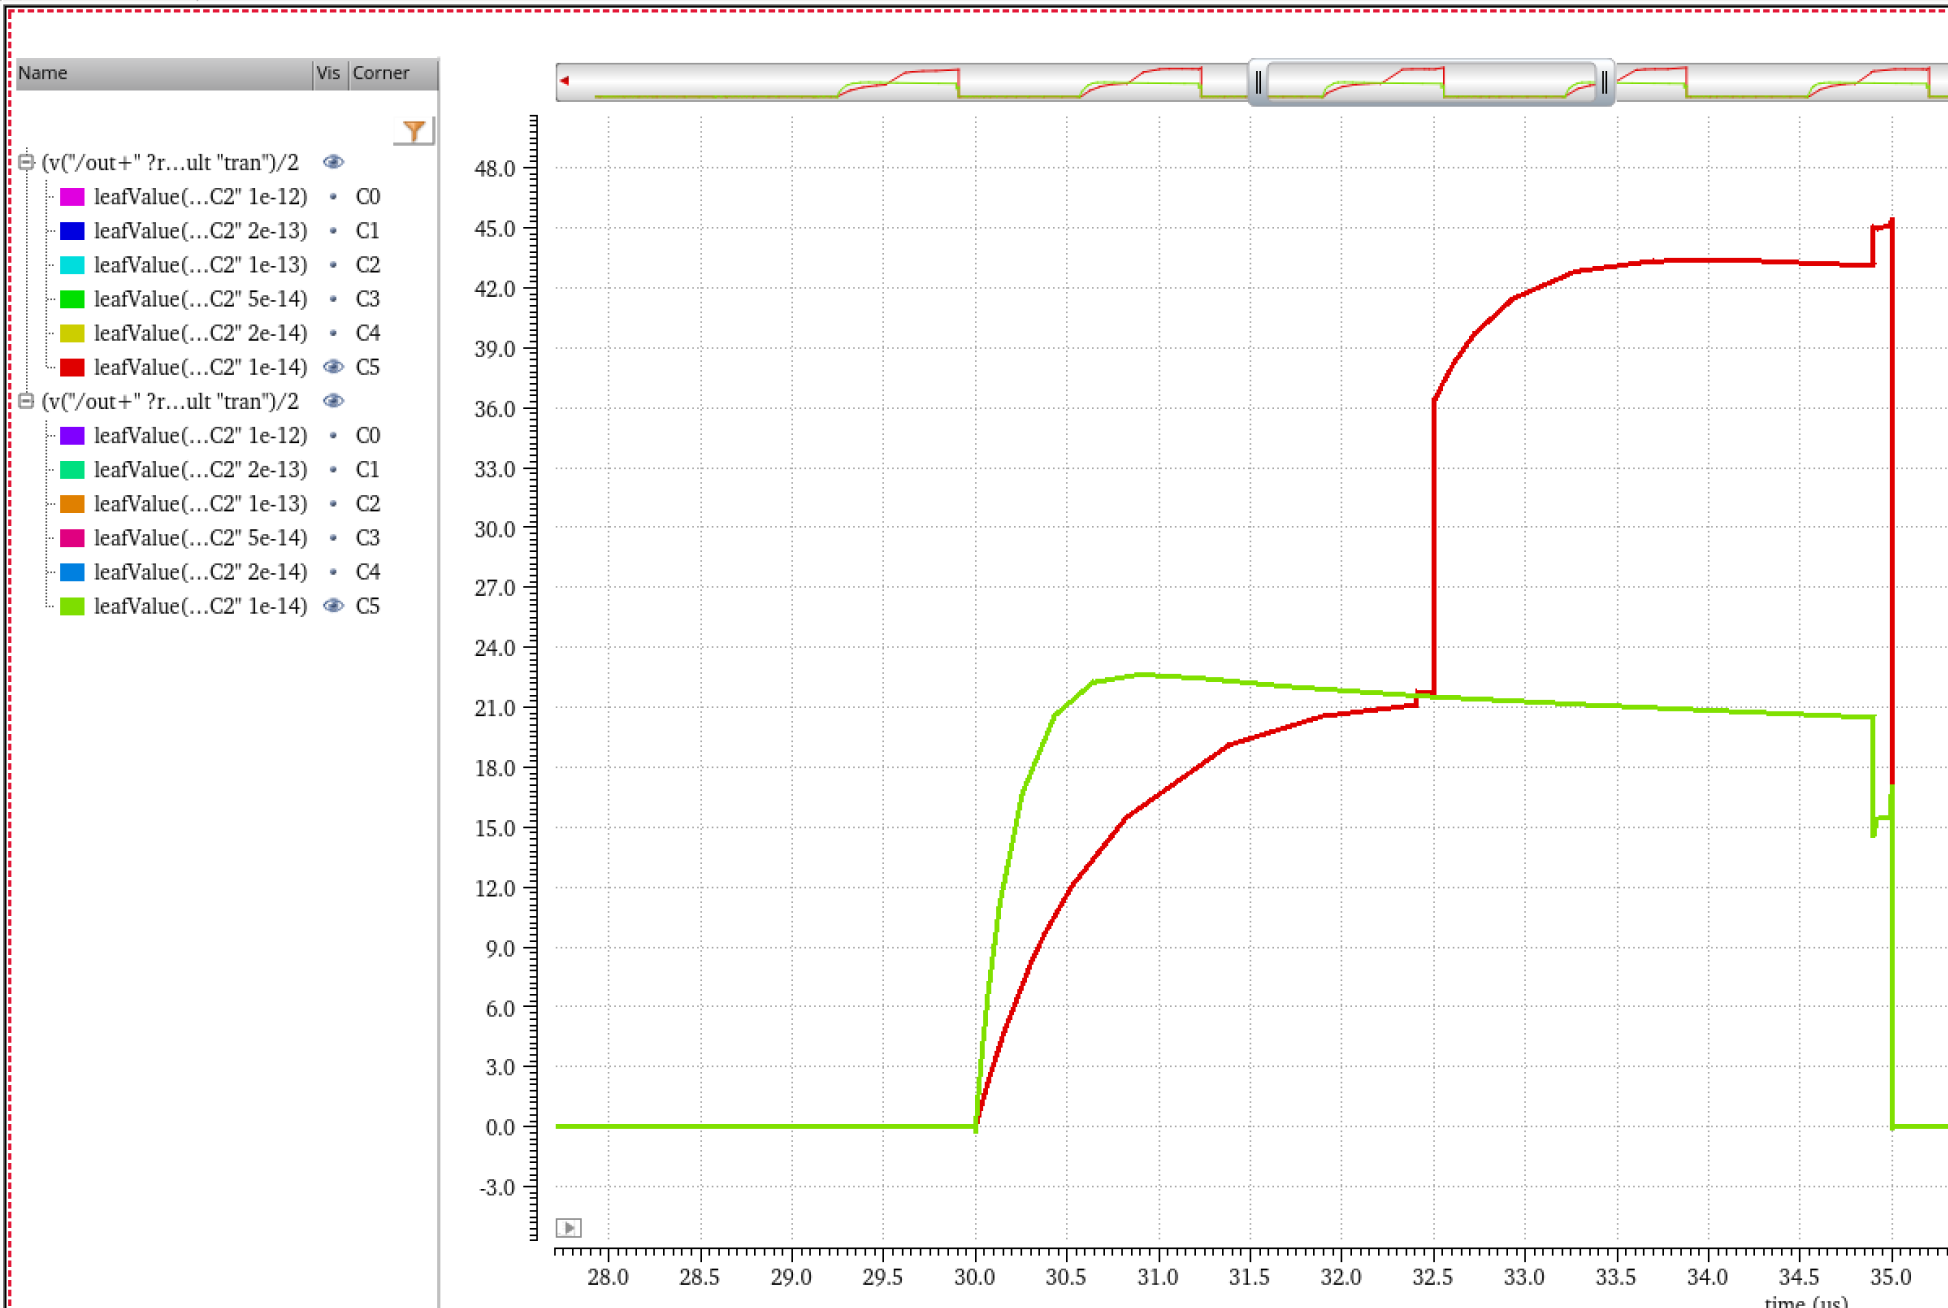
\includegraphics[width=0.8\textwidth]{doc_thesis/figs/04/瞬态仿真下有无CLS对比.png}
    \caption{\ptheadingfont{有无CLS下的瞬态响应对比}}
    \label{fig:有无CLS下的瞬态响应对比}
\end{figure}

\subsection{线性度}
在输入电压提升、输出电压提升时，由于输出电压无法超过电源电压，
因此LVFIA的输入输出电压会被压缩在电源轨附近，随着输出摆幅靠近电源轨，增益会显著下降，
产生非线性失真，导致整体电路的线性度下降。
引入CLS机制后，电平移位操作能够降低LVFIA的输出电压，从而减小非线性失真对整体输出的影响，
提升整体电路的线性度。通过不断改变动态放大器的输入幅度和输出幅度，我们对引入CLS机制前后的电路线性度进行了测试，
结果如表\ref{tab:CLS电路线性度测试}所示。



\begin{table}[htbp]
    \centering
    \caption{\ptheadingfont{CLS电路线性度测试}}
    \label{tab:CLS电路线性度测试}
    \begin{tabular}{|c|c|c|c|c|c|c|}
        \hline
         输出摆幅 & 42.53 & 84.71 & 126.65 & 168.01 & 208.78 & 248.05 \\
        \hline
        增益 & 42.63 & 42.44 & 42.31 & 42.11 & 41.88 & 41.54 \\
        \hline
    \end{tabular}
\end{table}
